\pdfinfoomitdate=1
\pdftrailerid{}
\pdfsuppressptexinfo=15
\documentclass[11pt]{article}
\usepackage[T1]{fontenc}
\usepackage{lmodern}
\usepackage[margin=1in]{geometry}
\usepackage{amsmath,amssymb,amsthm,mathtools}
\usepackage{microtype,graphicx,xcolor,tikz,enumitem,flafter}
\usetikzlibrary{arrows.meta,positioning,calc}
\usepackage[colorlinks=true,linkcolor=blue!45!black,citecolor=blue!45!black,urlcolor=blue!45!black]{hyperref}
\hypersetup{pdftitle={Translative covering densities of order n log n},pdfauthor={OpenAI}}
\newtheorem{theorem}{Theorem}[section]
\newtheorem{proposition}[theorem]{Proposition}
\newtheorem{lemma}[theorem]{Lemma}
\newtheorem{corollary}[theorem]{Corollary}
\theoremstyle{definition}
\newtheorem{definition}[theorem]{Definition}
\theoremstyle{remark}
\newtheorem{remark}[theorem]{Remark}
\numberwithin{equation}{section}
\DeclareMathOperator{\vol}{vol}
\setlist{itemsep=3pt,topsep=5pt}
\title{Translative covering densities of order $n\log n$}
\author{OpenAI}
\date{September 23, 2026}
\begin{document}
\maketitle
\begin{abstract}
For every sufficiently large dimension $n$, we construct a centrally symmetric
convex body whose translative covering density exceeds $c n\log n$,
where $c>0$ is absolute. This disproves the existence of a universal linear
upper bound and matches the order of Rogers' upper bound.
\end{abstract}
\tableofcontents
\clearpage
\section{Introduction}

A convex body in $\mathbb R^n$ is a compact convex set with nonempty interior.
A set $X\subset\mathbb R^n$ is \emph{locally finite} if every bounded set
contains only finitely many of its points. It gives a \emph{translative
covering} of $K$ when $K+X=\mathbb R^n$. Write $Q_R=[-R,R]^n$. We define
the translative covering density by
\begin{equation}\label{eq:unrestricted-density}
 \theta_T(K)=\inf_{\substack{X\text{ locally finite}\\K+X=\mathbb R^n}}
 \vol(K)\limsup_{R\to\infty}
       \frac{\#(X\cap Q_R)}{(2R)^n}.
\end{equation}
Thus the density measures the asymptotic volume of translates per unit
volume, counting overlaps. It is not the fraction of space covered, which
is one for every covering. No asymptotic density limit is assumed for an
individual arrangement.

A \emph{periodic translative covering} is a covering
\[
 \mathbb R^n=K+\Lambda+T,
\]
where $\Lambda$ is a full-rank lattice and $T$ is a finite set of distinct
representatives modulo $\Lambda$. Its center intensity is
$|T|/\det\Lambda$, and its density is $|T|\vol(K)/\det\Lambda$. Put
\[
 \theta_{\mathrm{per}}(K)=\inf\left\{
 \frac{|T|\vol(K)}{\det\Lambda}:K+\Lambda+T=\mathbb R^n
 \right\}.
\]
The infimum ranges over every lattice and every finite set $T$. In particular, there is no bound on the number of cosets.
Allowing repeated representatives of the same coset gives the same
infimum: deleting redundant representatives preserves the covering and
does not increase its listed density. When we later retain indexed center
lists, we count such repetitions explicitly.
Both infima are finite: an interior cube of $K$ gives a covering by
translates on a sufficiently fine cubic lattice.

The classical periodization principle gives
\begin{equation}\label{eq:density-equivalence}
 \theta_T(K)=\theta_{\mathrm{per}}(K).
\end{equation}
We prove the precise statement in Appendix~\ref{sec:periodization},
including agreement with lower or upper centered-ball density and average
covering multiplicity. See also Prosanov~\cite[Section~1.1 and
Theorem~2.1]{Prosanov2021PackingCovering}, who attributes the principle to
Rogers. These are equalities of optimal densities; the lower and upper
densities of an individual nonperiodic arrangement need not agree.

\begin{theorem}\label{thm:main}
There are absolute constants $c>0$ and $n_0$ such that, for every integer
$n\ge n_0$, some centrally symmetric convex body $K_n\subset\mathbb R^n$
satisfies
\[
 \theta_T(K_n)>c n\log n.
\]
\end{theorem}

Thus there is no absolute constant $C$ such that
$\theta_T(K)\le Cn$ for every convex body in every dimension, even if the
bodies are required to be centrally symmetric. This answers negatively
the universal linear-bound question recorded by
Nasz\'odi~\cite[Section~3]{Naszodi2018Flavors}.
Rogers~\cite{Rogers1957Coverings} proved that every convex body in dimension
$n\ge3$ has a periodic translative covering of density at most
\begin{equation}\label{eq:rogers}
 n\log n+n\log\log n+5n.
\end{equation}
Together with Theorem~\ref{thm:main}, this shows that the supremum of
covering density over convex bodies has order $n\log n$. The same order holds when
one restricts the bodies to be centrally symmetric. The constant in
Theorem~\ref{thm:main} is not optimized.
The bodies may moreover be chosen to be centrally symmetric polytopes
with rational vertices, with the same constant $c$; see
Corollary~\ref{cor:rational-polytope}.

\subsection{Antecedents and the additional uniformity}

Rogers' theorem supplies a universal upper bound for arbitrary convex
bodies. Fejes T\'oth~\cite{FejesToth2009Covering} sharpened its lower-order
term to obtain density
$n(\log n+\log\log n+1+o(1))$ using only $O(\log n)$ cosets of a common
lattice. A finite union of lattice cosets has substantially more freedom
than one lattice, even with this bound on the number of cosets.
On the lower-bound side, the classical work of Coxeter, Few and
Rogers~\cite{CoxeterFewRogers1959Spheres} gives an order-$n$ obstruction
already for unrestricted coverings by equal Euclidean balls.
For Euclidean balls, Dumer~\cite[Corollary~2]{Dumer2007Spheres} gives the
upper bound $(1/2+o(1))n\log n$. The gap for Euclidean balls remains;
our theorem determines the optimal order when the convex body may also
be chosen.

The proof builds on the random-slab construction and Poisson witness method
of Li and Liu~\cite[Theorem~1.3]{LiLiu2026Lattice}. They prove an order-$n\log n$ lower bound
for \emph{lattice} covering density, in which the centers form a single
lattice. Their common-intersection estimates, terminal clustering of caps,
and overlap-diagram bounds provide the local probabilistic machinery used
here. We give the necessary versions and their proofs, including the
continuous form of Janson's inequality.

The additional issue is to exclude every finite union of lattice cosets.
A net of lattice bases cannot encode an arbitrary number of cosets. We
instead localize an arrangement in a fixed Euclidean window, keeping every
center with its multiplicity, and round the resulting list to a finite grid.
Periodic averaging controls this list even when the lattice has very short
periods or a highly skew fundamental domain. The resulting finite class is
fixed before the body is sampled, so it includes arrangements chosen after
the body is known. A sufficiently strong lower-tail bound then excludes
all of them simultaneously.

For comparison, Bukh, Gao, Liu, Pikhurko, and Sun~\cite[Theorem~1.3]{BukhEtAl2025Random}
show that, in their packing-torus model, Poisson centers at a specified
density of order $n\log n$ fail to cover a given body with probability
tending to one.
Their random-centers barrier has different quantifiers: an exceptional arrangement might still
cover efficiently. Here the body is random and the conclusion excludes
every periodic arrangement for one realization of that body.

\subsection{Proof outline}

Intersect a slightly enlarged Euclidean ball with symmetric slabs whose unit
normals are sampled by a Poisson process.
The normalization gives this body a substantial volume with positive
probability. A hypothetical covering of low center intensity supplies,
after localization and rounding, a finite center list with many suitable
target points in a small window. We must show that each such list is very
unlikely to cover that window.

At a target $y$, only centers $p$ within the outer ball's radius of $y$
can cover it. For each such center, the residual vector $y-p$ determines
the antipodal caps of slab normals that would remove $y$ from that
translate. A hole appears if the Poisson process hits at least one cap
in each pair. Nearly coincident cutting sets are strongly dependent.
Following Li and Liu, we group these conditions into blocks and choose one common subset of normals
for each block. Assigning distinct Poisson points to these subsets certifies
a hole. The block construction controls the complete overlap sum of these
certificates, including their self-overlaps.

The targets are chosen at two angular scales. For every pair of distinct
targets, every pair of their relevant residual directions is separated
at a scale of order $\sqrt{\log n/n}$, identifying opposite directions
because the slabs are symmetric. The cap estimates then bound the
dependence between their hole certificates. The body lies in a ball
whose radius is only slightly larger than the slab half-width, so its
cutting caps have a small fixed angular radius. At a larger fixed
separation, all cutting caps belonging to one target are disjoint from
those belonging to the other. A cylinder-volume estimate lets us arrange
this stronger separation for all but an exponentially small fraction of
target pairs, while retaining the finer separation for every pair.

Let $R$ denote the density lower bound sought. We can choose
$\exp(c_1n\log n)$ targets for a fixed $c_1>0$, enough to absorb a
self-overlap cost $\exp(CR)$ when $R=c n\log n$ and $c$ is sufficiently
small. The two angular scales control the remaining overlap between
distinct targets. Janson's lower-tail inequality turns these bounds into
a covering probability that is doubly exponentially small in $n$, with
decay strong enough to dominate the number of rounded patterns.
A second-moment bound would not give the required decay.

Section~\ref{sec:construction} defines the body and the constants.
Section~\ref{sec:localization} constructs the finite pattern class.
Sections~\ref{sec:caps}--\ref{sec:poisson} establish the cap, block, and
Poisson estimates. Section~\ref{sec:targets} proves the fixed-pattern bound,
and Section~\ref{sec:assembly} completes the proof.
Section~\ref{sec:encoding} gives rational-polytope and rational-normal
versions of the construction.
Appendix~\ref{sec:periodization} proves the density equivalence that
transfers the periodic exclusion to unrestricted coverings.

\subsection{Notation}

Logarithms are natural, and $[t]_+=\max\{t,0\}$. We write $|x|$ for Euclidean norm,
$B_r=\{x\in\mathbb R^n:|x|\le r\}$, $B=B_1$, and
$\omega_n=\vol(B)$. For measurable sets in $\mathbb R^n$, $|A|$ also denotes
Lebesgue volume; for finite lists and index sets it denotes cardinality.
Surface measure $\sigma$ on $S^{n-1}$ is normalized to have total mass one.
For nonzero vectors we use the projective angle
\[
 \angle(x,z)=\arccos\frac{|x\cdot z|}{|x||z|}\in[0,\pi/2].
\]
Lists are indexed: two entries can occupy the same point or define the same
cap. Every sum and cardinality over such a list retains its multiplicities.
Constants implicit in $O(\cdot)$ depend only on parameters explicitly fixed
before $n$ tends to infinity.

\section{The random body}\label{sec:construction}

Fix the numerical constants
\begin{equation}\label{eq:fixed-constants}
 \varepsilon=2^{-30},\qquad a=1+\varepsilon,\qquad
 D=2^{-10}=\varepsilon^{1/3},\qquad v=\frac1{64}.
\end{equation}
For each sufficiently large $n$, put
\begin{equation}\label{eq:radii}
 \eta=n^{-4},\qquad b=a(1+1/n),\qquad
 r_-=a(1-10\log n/n).
\end{equation}
The small window is $B_D$. Its size relative to $a$ will govern the number
of patterns, through
\begin{equation}\label{eq:rates}
 \lambda_0=\log(1+D/a),\qquad
 \gamma=\log\frac{D}{8\sqrt\varepsilon}-2\lambda_0
        =\log4-2\lambda_0.
\end{equation}
Since $\lambda_0<D=2^{-10}$, we have $\gamma>3\lambda_0$.
These constants are fixed; none tends to zero with dimension.

Set
\begin{equation}\label{eq:poisson-measure}
 M=\bigl(\sigma\{u:|u\cdot e_1|>1/a\}\bigr)^{-1},\qquad \mu=M\sigma,
\end{equation}
and let $\Pi$ be a Poisson process on $S^{n-1}$ with intensity $\mu$.
Equivalently, sample a Poisson random integer of mean $M$, then that many
independent $\sigma$-distributed unit normals. Define
\begin{align}
 K&=bB\cap\bigcap_{u\in\Pi}\{x:|u\cdot x|\le1\},\label{eq:body}\\
 K^+&=(b+3\eta)B\cap\bigcap_{u\in\Pi}\{x:|u\cdot x|\le1+3\eta\}.
 \label{eq:buffered-body}
\end{align}
The enlarged body $K^+$ absorbs the displacement of centers during rounding.
Since $M<\infty$, the list of normals is finite almost surely. Both bodies
are compact and centrally symmetric, and $B\subset K$, so $K$ has nonempty
interior.

\begin{lemma}\label{lem:volume}
The body in~\eqref{eq:body} satisfies
\[
 \mathbb P\{|K|>2v\omega_n a^n\}
 \ge \frac{\exp(-1)-2v}{3-2v}>0.
\]
\end{lemma}
\begin{proof}
If $|x|\le a$, the $\mu$-measure of normals with $|u\cdot x|>1$ is at
most one by rotational invariance and~\eqref{eq:poisson-measure}. The
probability that there is no such Poisson normal is therefore at least
$\exp(-1)$. Integrating over $aB$ gives
$\mathbb E|K|\ge\exp(-1)\omega_n a^n$.
On the other hand, $|K|\le\omega_n b^n<3\omega_n a^n$. Thus
$X=|K|/(\omega_n a^n)$ has $0\le X\le3$ and $\mathbb E X\ge\exp(-1)$.
Writing $p=\mathbb P(X>2v)$, we have
$\mathbb E X\le2v(1-p)+3p$, which proves the claim.
\end{proof}

We shall rule out coverings with center intensity at most
\begin{equation}\label{eq:intensity-threshold}
 \rho_0=\frac{R}{2v\omega_n a^n},
\end{equation}
where $R$ is a positive parameter. This threshold does not depend on the
realized volume. Once every such covering is excluded, the definition of
$\theta_{\mathrm{per}}$ gives $\theta_{\mathrm{per}}(K)\ge\rho_0|K|$. The strict volume event in
Lemma~\ref{lem:volume} will then imply $\theta_{\mathrm{per}}(K)>R$, including strictness
at the infimum.

\section{Reducing all periodic coverings to finitely many patterns}
\label{sec:localization}

We first remove the lattice and its fundamental domain from the subsequent
probability estimate.  A periodic arrangement of bounded center intensity
has a translated ball containing relatively few centers and many points
with controlled residual vectors.  Rounding those centers produces a list
in a fixed finite family.  The argument counts every occurrence of a center,
so it applies to arbitrarily short or skew periods and to coinciding cosets.

Use the fixed parameters $a,D,v,b,r_-,\eta$ from the preceding section,
and let $1\le R\le n^2$.  Define
\[
 C_{\mathrm{loc}}=\frac{1000}{v},\qquad
 w_a(r)=1+n[1-r^2/a^2]_+ \quad (r\ge0),
 \qquad h_n=\frac{\eta}{100n}.
\]
The weight $w_a$ records the radial cost of a center near a target point.
Our finite alphabet and maximum list length are
\begin{equation}\label{eq:local-grid}
 \mathcal Q_n=h_n\mathbb Z^n\cap B_{D+b+5\eta},\qquad
 N_n=\left\lceil\frac{20R}{v}
       \left(\frac{D+b+5\eta}{a}\right)^n\right\rceil.
\end{equation}
An ordered list $P=(p_1,\ldots,p_m)$ over $\mathcal Q_n$ may contain repeated
entries.  Define $G_P\subseteq B_D$ to consist of the points $y$ satisfying
the following three conditions:
\begin{align}
 |y-p_j|&\ge r_--2\eta &&(1\le j\le m),\label{eq:rounded-inner}\\
 \#\{j:|y-p_j|\le b+3\eta\}&\le2C_{\mathrm{loc}}R,
       \label{eq:rounded-count}\\
 \sum_{j:\,|y-p_j|\le b+3\eta}w_a(|y-p_j|)
       &\le2C_{\mathrm{loc}}R.\label{eq:rounded-weight}
\end{align}
The count condition follows from the weight condition because $w_a\ge1$;
we display both to identify the cardinality and cost bounds used later.
All sums count indices, including repeated entries.  Set
\begin{equation}\label{eq:pattern-family}
 \mathcal F_n=
 \left\{P\in\bigcup_{m=0}^{N_n}\mathcal Q_n^m:
              |G_P|\ge\frac14|B_D|\right\}.
\end{equation}
The dependence of $N_n$ and $\mathcal F_n$ on $R$ is suppressed in the
notation.  Empty lists are allowed, with all their sums equal to zero.

\begin{proposition}[Deterministic localization]\label{prop:localization}
For all sufficiently large $n$, uniformly for $1\le R\le n^2$, the family
$\mathcal F_n$ has the following properties.  With
$\lambda_0=\log(1+D/a)$,
\begin{equation}\label{eq:pattern-entropy}
 N_n\le n^{C_1}\exp(\lambda_0n),\qquad
 \log|\mathcal F_n|
       \le\exp\bigl(\lambda_0n+O(\log n)\bigr),
\end{equation}
where $C_1$ and the implicit constant depend only on the fixed parameters.

Let $\mathcal U\subset S^{n-1}$ be any finite set, and put
\[
 K=bB\cap\bigcap_{u\in\mathcal U}\{x:|u\cdot x|\le1\},\qquad
 K^+=(b+3\eta)B\cap
          \bigcap_{u\in\mathcal U}\{x:|u\cdot x|\le1+3\eta\}.
\]
Suppose that $\Lambda$ is any full-rank lattice, $T\subset\mathbb R^n$
is finite, and
\[
 \frac{|T|}{\det\Lambda}\le
       \rho_0:=\frac{R}{2v\omega_na^n}.
\]
If $K+\Lambda+T$ covers $\mathbb R^n$, there is a list
$P=(p_1,\ldots,p_m)\in\mathcal F_n$
such that
\begin{equation}\label{eq:localized-cover}
 B_D\subseteq\bigcup_{j=1}^{m}(p_j+K^+).
\end{equation}
The constructed list in fact satisfies $|G_P|\ge|B_D|/2$.

For every $P\in\mathcal F_n$ and $y\in G_P$, list all residual vectors
$x_i=y-p_j$ with $|y-p_j|\le b+3\eta$, retaining their indices, and denote
their number by $m_y$.  Then
\begin{equation}\label{eq:local-residual-budget}
 \begin{gathered}
 r_--2\eta\le |x_i|\le b+3\eta,\qquad
 m_y\le2C_{\mathrm{loc}}R,\qquad
 \sum_{i=1}^{m_y}w_a(|x_i|)\le2C_{\mathrm{loc}}R,\\
 m_y+\sum_{i=1}^{m_y}w_a(|x_i|)\le4C_{\mathrm{loc}}R.
 \end{gathered}
\end{equation}
\end{proposition}

\begin{proof}
We prove the localization and rounding assertions first, then count the
resulting lists.  All dimension thresholds in the proof are uniform for
$1\le R\le n^2$.

\paragraph{Averaging the full multiset of centers.}
Give each center an index $(t,\ell)\in T\times\Lambda$, at position
$t+\ell$.  Distinct indices remain distinct even if they have the same
position.  This multiset is locally finite because $T$ is finite and
$\Lambda$ is discrete.  Write $\rho=|T|/\det\Lambda$, and let $F$ be a
fundamental parallelepiped of $\Lambda$.  For every nonnegative integrable
function $f$,
\begin{equation}\label{eq:periodic-averaging}
 \frac1{|F|}\int_F
       \sum_{(t,\ell)\in T\times\Lambda} f(y-t-\ell)\,dy
       =\rho\int_{\mathbb R^n}f(x)\,dx.
\end{equation}
Indeed, Tonelli's theorem permits the sums to be interchanged with the
integral.  For each $t$, the sets $F-t-\ell$, $\ell\in\Lambda$, partition
$\mathbb R^n$ up to null sets.  This proves the identity without any
restriction on the shape or size of $F$.

Put $\beta=b+4\eta$.  Call a point $y\in\mathbb R^n$ unrounded-good if
there is no center occurrence at distance less than $r_-$, at most
$C_{\mathrm{loc}}R$ occurrences have distance at most $\beta$, and
\begin{equation}\label{eq:unrounded-weight}
 \sum_{(t,\ell):\,|y-t-\ell|\le\beta}
         w_a(|y-t-\ell|)\le C_{\mathrm{loc}}R.
\end{equation}
Let $G$ be this periodic measurable set.  These conditions respectively
exclude short residuals, bound the number of relevant residuals, and bound
their total radial cost.  Using the full ball ensures that every index
entering a rounded test is counted before rounding.

For a uniform point modulo $\Lambda$, the expected number of occurrences
in its open $r_-$-ball is at most
\[
 \rho\omega_n r_-^n
 \le\frac{R}{2v}
       \left(1-\frac{10\log n}{n}\right)^n
 \le\frac{R n^{-10}}{2v}
 \le\frac1{200}
\]
for large $n$.  Hence the first condition fails with probability at most
$1/200$.  Also
\[
 \left(\frac\beta a\right)^n
 \le\exp(1+4/n^3)<3
\]
for large $n$, so the expected outer count is at most $3R/(2v)$.
For the weighted condition, polar integration gives the exact identity
\begin{align}
 \int_{B_\beta}w_a(|x|)\,dx
 &=\omega_n\beta^n
      +n\int_{B_a}(1-|x|^2/a^2)\,dx\notag\\
 &=\omega_n\beta^n+\frac{2n}{n+2}\omega_na^n
 <5\omega_na^n.\label{eq:weighted-ball-integral}
\end{align}
Equation \eqref{eq:periodic-averaging} therefore bounds the expected
weighted sum by $5R/(2v)$.  Markov's inequality bounds the two remaining
failure probabilities by $3/2000$ and $5/2000$, respectively.  Consequently
\begin{equation}\label{eq:periodic-good-volume}
 \frac{|G\cap F|}{|F|}
 \ge1-\frac1{200}-\frac3{2000}-\frac5{2000}
 >\frac{99}{100}.
\end{equation}

\paragraph{One window with both required bounds.}
For $z$ uniform modulo $\Lambda$, let $M(z)$ count all center occurrences
in $z+B_{D+b+4\eta}$.  Equations \eqref{eq:periodic-averaging} and
\eqref{eq:local-grid} imply
\[
 \mathbb{E} M(z)
 \le\frac{R}{2v}\left(\frac{D+b+4\eta}{a}\right)^n
 \le\frac{N_n}{40}.
\]
Moreover, periodicity and Fubini's theorem give
\[
 \mathbb{E}\frac{|(z+B_D)\setminus G|}{|B_D|}
 =1-\frac{|G\cap F|}{|F|}\le\frac1{100}.
\]
Both expressions concern the entire Euclidean window, including all its
overlapping period copies.  Markov's inequality gives
\[
 \mathbb{P}\{M(z)>N_n\}\le\frac1{40},\qquad
 \mathbb{P}\{|(z+B_D)\setminus G|>|B_D|/2\}\le\frac1{50}.
\]
The sum is less than one.  Fix a slide $z$ outside these two exceptional
events, and retain every occurrence in $z+B_{D+b+4\eta}$.  There are at
most $N_n$ such occurrences, and at least half of $z+B_D$ lies in $G$.

\paragraph{Rounding and transferring coverage.}
Translate this window and the retained centers by $-z$, and round every
center coordinatewise to the nearest point of $h_n\mathbb Z^n$, using a
fixed rule for ties.  Each center moves a distance at most
\begin{equation}\label{eq:rounding-error}
 \delta_n=\frac{\sqrt n h_n}{2}
         =\frac{\eta}{200\sqrt n}\le\frac\eta{200}.
\end{equation}
The rounded centers belong to $\mathcal Q_n$; enumerate them as an ordered
list $P$, retaining all repeated entries.

We check that every $y\in B_D$ with $y+z\in G$ belongs to $G_P$.
Every unrounded residual has length at least $r_-$, so every rounded one
has length at least $r_--\delta_n\ge r_--2\eta$.
A rounded residual of length at most $b+3\eta$ comes from an unrounded
residual of length at most
\[
 b+3\eta+\delta_n<b+4\eta.
\]
Thus at most $C_{\mathrm{loc}}R$ rounded indices are relevant.  This
strict separation of the two outer radii ensures that every index entering
a rounded test was counted before rounding.

The function $w_a$ is globally Lipschitz on $[0,\infty)$ with constant
$2n/a$.  Its derivative has absolute value $2nr/a^2\le2n/a$ for
$0<r<a$, and it is constant for $r>a$.  If $r$ and $r'$ are the
unrounded and rounded lengths of a relevant residual, then
\[
 w_a(r')\le w_a(r)+\frac{2n\delta_n}{a}
          \le\left(1+\frac{2n\delta_n}{a}\right)w_a(r),
\]
where the last step uses $w_a(r)\ge1$.  Summing over the relevant indices,
all of which were included in \eqref{eq:unrounded-weight}, gives
\[
 \sum_{j:\,|y-p_j|\le b+3\eta}w_a(|y-p_j|)
 \le\left(1+\frac{2n\delta_n}{a}\right)C_{\mathrm{loc}}R
 \le2C_{\mathrm{loc}}R.
\]
This verifies \eqref{eq:rounded-inner}--\eqref{eq:rounded-weight}.
In particular, $|G_P|\ge|B_D|/2$ and $P\in\mathcal F_n$.

Now assume that the original periodic arrangement covers by $K$.
For any point of $z+B_D$, every center whose translate of $K$ contains
that point lies in $z+B_{D+b}$ because $K\subseteq bB$.  Such a center was
retained.  Moving it by at most $\delta_n$ changes the residual norm by at
most $\delta_n$ and each scalar product with a unit normal by at most
$\delta_n$.  Hence its rounded translate of $K^+$ contains the translated
point of $B_D$.  This proves \eqref{eq:localized-cover} for every point of
the closed window.

\paragraph{Counting the lists.}
Write $J_n=|\mathcal Q_n|$.  A containing cube gives
\[
 J_n\le\left(1+\frac{2(D+b+5\eta)}{h_n}\right)^n,
 \qquad \log J_n=O(n\log n).
\]
Since $b=a(1+1/n)$, $\eta=n^{-4}$, and $1\le R\le n^2$,
\[
 \log N_n=\lambda_0n+O(\log n).
\]
This proves the first bound in \eqref{eq:pattern-entropy}.  Counting ordered
lists allows all multiplicities and gives
\[
 |\mathcal F_n|\le\sum_{m=0}^{N_n}J_n^m
       \le(N_n+1)J_n^{N_n}.
\]
The two preceding estimates give the second bound in
\eqref{eq:pattern-entropy}.
Finally, \eqref{eq:local-residual-budget} follows directly from the
definition of $G_P$ and $w_a\ge1$.
\end{proof}

The family $\mathcal F_n$ depends only on the fixed numerical parameters,
$n$, and $R$.  Proposition~\ref{prop:localization} holds for every choice
of the slab normals and every periodic covering of the required intensity.
Thus a probability bound uniform over this finite family also controls
centers chosen after the body is known.  The next sections obtain such a
bound by finding a point of $G_P$ missed by all translates in a fixed list.

\section{Intersections of spherical caps}
\label{sec:caps}

We need two properties of the cutting caps: separated caps have small
overlap, whereas a collection of nearby caps has a substantial common
intersection. For a target $y\in G_P$ and a relevant center $p$, write
$x=y-p$. The set
\[
 C(x)=\{u\in S^{n-1}:|u\cdot x|>1+3\eta\}
\]
consists of the normals whose slabs exclude $y$ from $p+K^+$.
Figure~\ref{fig:residual-cap} illustrates this correspondence. The
estimates below allow the slightly more general thresholds needed to
control these caps uniformly.
\begin{figure}[htbp]
\centering
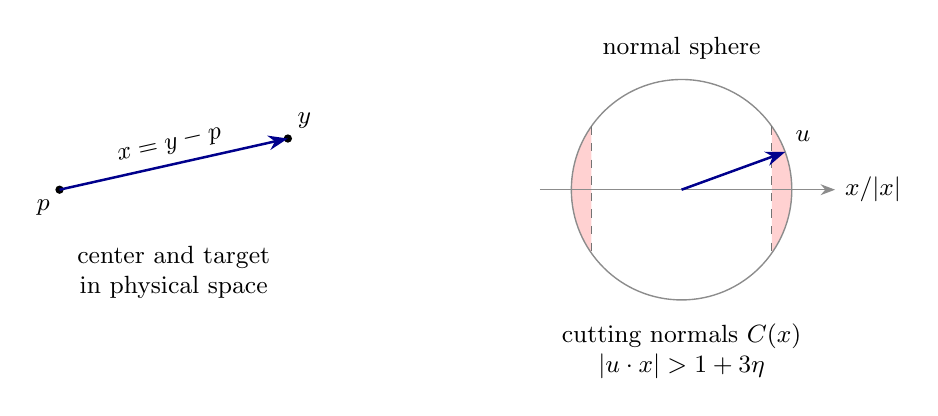
\begin{tikzpicture}[x=1cm,y=1cm,>=Stealth,
 every node/.style={font=\small},
 axis/.style={draw=black!45,line width=.5pt},
 vector/.style={->,draw=blue!55!black,line width=.9pt}]
 \coordinate (p) at (0,0);
 \coordinate (y) at (2.9,.65);
 \fill (p) circle (1.5pt) node[below left] {$p$};
 \fill (y) circle (1.5pt) node[above right] {$y$};
 \draw[vector] (p) -- (y) node[midway,above,sloped] {$x=y-p$};
 \node[align=center] at (1.45,-1.05) {center and target\\in physical space};

 \begin{scope}[shift={(7.9,0)}]
  \fill[red!18] (35:1.4) arc (35:-35:1.4) -- cycle;
  \fill[red!18] (145:1.4) arc (145:215:1.4) -- cycle;
  \draw[axis] (0,0) circle (1.4);
  \draw[axis,->] (-1.8,0) -- (1.95,0) node[right] {$x/|x|$};
  \draw[dashed,black!55] (35:1.4) -- (-35:1.4);
  \draw[dashed,black!55] (145:1.4) -- (215:1.4);
  \draw[vector] (0,0) -- (20:1.4) node[above right] {$u$};
  \node[align=center] at (0,-2.05)
    {cutting normals $C(x)$\\$|u\cdot x|>1+3\eta$};
  \node at (0,1.8) {normal sphere};
 \end{scope}
\end{tikzpicture}
\caption{Plane-section schematic of a residual and its cutting cap.
The shaded antipodal caps lie beyond the two threshold hyperplanes
$u\cdot x=\pm(1+3\eta)$. A sampled normal in $C(x)$ excludes the target
$y$ from $p+K^+$. The drawing does not depict high-dimensional cap
measure. For a block of residuals, one normal in their common subset
cuts them all; assigning distinct normals to all blocks is a sufficient
certificate of a hole.}
\label{fig:residual-cap}
\end{figure}


The estimates adapt Li--Liu's cap and common-lens
arguments \cite[Lemma~6.1 and Lemmas~9.2--9.3]{LiLiu2026Lattice}.
In our thin radial shell, a bisector argument gives a short proof of the
overlap estimate with a constant prefactor. Keeping that prefactor
independent of dimension will be important when we sum overlaps.

\begin{lemma}[Cap estimates]\label{lem:caps}
Fix \(1<a<2\) and \(A,Q,B_0>0\). There exist constants
\(C_a,c_a'>0\), \(C_{a,A}>0\), and \(L=L(a)>0\) such that the
following holds for all sufficiently large \(n\), depending on
\(a,A,Q,B_0\). Let \(\sigma\) be normalized surface measure on
\(S^{n-1}\), and set
\[
 M=\sigma\{u:|u\cdot e_1|>1/a\}^{-1},\qquad \mu=M\sigma.
\]
Let \(x_1,\ldots,x_m\in\mathbb{R}^n\) and
\(\epsilon_1,\ldots,\epsilon_m\in\mathbb{R}\), where
\(1\le m\le n^2\), satisfy
\[
 a\left(1-\frac{A\log n}{n}\right)-Qn^{-4}
 \le |x_i|\le a(1+1/n)+Qn^{-4},\qquad
 |\epsilon_i|\le Qn^{-4}.
\]
Define
\[
 C_i=\{u\in S^{n-1}:|u\cdot x_i|>1+\epsilon_i\},\quad
 c_i=\mu(C_i),\quad \bar c_i=\min(c_i,1/2),\quad
 s_i=-\log\bar c_i,
\]
and, using projective angles, define
\[
 d(i,j)=\sqrt n\,\angle(x_i,x_j)+\sqrt{|s_i-s_j|},\qquad
 r(S)=\min_{k\in S}\max_{i\in S}d(k,i)^2
\]
for each nonempty set \(S\) of indices. Then
\begin{align}
 n^{-C_{a,A}}\le c_i&\le C_a,
 &s_i&\le C_a\bigl(1+n[1-|x_i|^2/a^2]_+\bigr),
 \label{eq:caps-cost}\\
 \frac{\mu(C_i\cap C_j)}{\sqrt{\bar c_i\bar c_j}}
 &\le C_a\exp\{-c_a'd(i,j)^2\}.
 \label{eq:caps-affinity}
\end{align}
The function \(d\) is a pseudometric on the indexed list. If
\(r(S)\le B_0\log n\) and \(i_0\in S\) minimizes the raw intensity
\(c_i\), then
\begin{equation}
 \mu\left(\bigcap_{i\in S}C_i\right)
 \ge e^{-L(1+r(S)+\log|S|)}\bar c_{i_0}.
 \label{eq:caps-lens}
\end{equation}
In particular, \(L\) is independent of \(A,Q,B_0\); these parameters
may affect the starting dimension.
\end{lemma}

\begin{proof}
We first record one-dimensional estimates, then prove the overlap and
common-intersection bounds. Constants with a subscript \(a\) below may
change from line to line, but depend only on \(a\).

\paragraph{One-cap probabilities and radial costs.}
Write \(t_*=1/a\), \(e_i=x_i/|x_i|\), and
\(\tau_i=(1+\epsilon_i)/|x_i|\). For a unit vector \(e\), let
\[
 F_n(t)=\sigma\{u:u\cdot e>t\}
 =k_n\int_t^1(1-v^2)^{(n-3)/2}\,dv,\qquad 0<t<1,
\]
where \(k_n\) is the normalization constant. Substitution of
\(z=1-v^2\), using \(1\le1/v\le1/t\), gives
\begin{equation}
 \frac{k_n}{n-1}(1-t^2)^{(n-1)/2}
 \le F_n(t)\le
 \frac{k_n}{(n-1)t}(1-t^2)^{(n-1)/2}.
 \label{eq:caps-mills}
\end{equation}
Consequently,
\begin{equation}
 \frac{(n-1)t}{1-t^2}
 \le-\frac{d}{dt}\log F_n(t)
 \le\frac{n-1}{1-t^2}.
 \label{eq:caps-hazard}
\end{equation}
These exact inequalities avoid dimension-dependent prefactors in
ratios of cap probabilities.

All the thresholds satisfy
\begin{equation}
 \tau_i=t_*+O_{a,A,Q}(\log n/n),\qquad
 \tau_i\ge t_*-C_a/n,
 \label{eq:caps-thresholds}
\end{equation}
for sufficiently large \(n\), and hence belong to the fixed interval
\(J=[t_*/2,(1+t_*)/2]\subset(0,1)\).
Since \(M=(2F_n(t_*))^{-1}\), we have
\(c_i=F_n(\tau_i)/F_n(t_*)\).
The logarithmic derivative in \eqref{eq:caps-hazard} is bounded by
\(C_an\) on \(J\). This proves \(c_i\le C_a\), while the lower radial
bound proves \(c_i\ge n^{-C_{a,A}}\).
More explicitly, putting \(\delta_i=[1-|x_i|^2/a^2]_+\), elementary
algebra gives
\[
\begin{gathered}
 (\tau_i-t_*)_+\le C_a(\delta_i+Qn^{-4}),\qquad
 (t_*-\tau_i)_+\le C_a(n^{-1}+Qn^{-4}),\\
 n\delta_i\le C_{a,A}\log n+O_{a,Q}(n^{-3}).
\end{gathered}
\]
Integrating \eqref{eq:caps-hazard} therefore gives
\(-\log c_i\le C_a(1+n\delta_i)\), after increasing the starting
dimension so that \(Qn^{-3}\le1\). As
\(s_i=\max(\log2,-\log c_i)\), this proves
\eqref{eq:caps-cost}. The additive constant is needed even when
\(c_i\ge1/2\).

\paragraph{The overlap bound.}
Consider two ordinary half caps with thresholds \(\tau,\upsilon\)
drawn from our list and with axis angle \(\theta\in[0,\pi]\).
Put \(t=(\tau+\upsilon)/2\). If \(\theta<\pi\), adding their two
defining inequalities shows that their intersection lies in the half
cap along the angle bisector with threshold
\[
 q=t/\cos(\theta/2).
\]
The intersection is empty if \(\theta=\pi\) or \(q\ge1\), so suppose
\(q<1\). Let \(f(z)=\log(1-z^2)\). Its second derivative is bounded
in absolute value on \(J\), whence
\[
 f(t)-\tfrac12 f(\tau)-\tfrac12 f(\upsilon)
 \le C_a(\tau-\upsilon)^2.
\]
Furthermore,
\[
 \frac{1-q^2}{1-t^2}
 =1-\frac{t^2}{1-t^2}\tan^2(\theta/2)
 \le e^{-c_a'\theta^2},
\]
using \(t\ge t_*/2\) and \(\tan(\theta/2)\ge\theta/2\).
Apply the upper bound in \eqref{eq:caps-mills} to \(F_n(q)\) and
the lower bound to both terms in the following denominator:
\begin{equation}
 \frac{F_n(q)}{\sqrt{F_n(\tau)F_n(\upsilon)}}
 \le q^{-1}\exp\{C_an(\tau-\upsilon)^2-c_a'n\theta^2\}
 \le C_a e^{-c_a'n\theta^2}.
 \label{eq:caps-bisector}
\end{equation}
Indeed, \(q^{-1}\le2/t_*\), and
\(n(\tau-\upsilon)^2=O_{a,A,Q}((\log n)^2/n)\to0\) by
\eqref{eq:caps-thresholds}. This last fact is the benefit of the
thin shell. The argument does not require \(q\in J\), so it also
applies when the bisector threshold approaches 1.

For projective angle \(\phi=\angle(x_i,x_j)\), the four pairs of
signed half caps have ordinary angles \(\phi\) or
\(\pi-\phi\ge\phi\). Summing \eqref{eq:caps-bisector} over these
four disjoint sign choices and using \(c_i=2MF_n(\tau_i)\) gives
\[
 \mu(C_i\cap C_j)\le C_a\sqrt{c_ic_j}\,e^{-c_a'n\phi^2}.
\]
By \eqref{eq:caps-cost}, \(c_i/\bar c_i\le\max(1,2C_a)\), so
clipping the denominator costs only a constant. Independently, the
trivial intersection bound gives
\[
 \frac{\mu(C_i\cap C_j)}{\sqrt{\bar c_i\bar c_j}}
 \le C_a e^{-|s_i-s_j|/2}.
\]
To see this, order the clipped intensities as
\(\bar c_i\le\bar c_j\). If \(\bar c_i<1/2\), use
\(\mu(C_i\cap C_j)\le c_i=\bar c_i\); otherwise both clipped
intensities equal \(1/2\), and use \(c_i\le C_a\).
The minimum of the two bounds is at most their geometric mean.
Together with
\[
 d(i,j)^2\le2\bigl(n\phi^2+|s_i-s_j|\bigr),
\]
this proves \eqref{eq:caps-affinity}.

Projective angle satisfies the triangle inequality, as the quotient
of spherical distance under antipodal identification. The inequality
\(\sqrt{x+y}\le\sqrt x+\sqrt y\) shows that
\(\sqrt{|s_i-s_j|}\) also satisfies it. Thus \(d\) is a
pseudometric; distinct labels, including repeated caps, may have
distance zero.

\paragraph{A common intersection.}
Set \(r=r(S)\) and \(m_S=|S|\), and choose an index attaining the
minimum defining \(r\). By the triangle inequality, each axis in
\(S\) has projective angle at most \(2\sqrt{r/n}\) from
\(e_0=e_{i_0}\). Since \(F_n\) is strictly decreasing, the
raw-minimum anchor has the largest threshold:
\(\tau_0=\tau_{i_0}\ge\tau_i\).
Orient each axis so that its ordinary angle \(\phi_i\) with
\(e_0\) equals its projective angle, and write
\[
 e_i=(\cos\phi_i)e_0+(\sin\phi_i)v_i,\qquad
 \Phi=\max_{i\in S}\phi_i\le2\sqrt{r/n},
\]
where \(v_i\) is a unit tangent vector. For \(\phi_i=0\), its
choice is immaterial.

We use the elementary bound
\begin{equation}
 \mathbb{P}(W\cdot v<-h)\le e^{-dh^2/2}
 \label{eq:caps-tangent}
\end{equation}
for a uniform \(W\in S^{d-1}\), \(d\ge2\), any unit \(v\), and
\(h\ge0\). Here is a proof. Rotational invariance reduces to
\(X=W_1\). Integrating the derivative of
\(x^{2j-1}(1-x^2)^{(d-1)/2}\) on \([-1,1]\) shows that
\[
 \mathbb{E} X^{2j}
 =\frac{2j-1}{d+2j-2}\mathbb{E} X^{2j-2}
 \le\frac{(2j)!}{2^j j!d^j}.
\]
Odd moments vanish. The exponential series therefore gives
\(\mathbb{E} e^{zX}\le e^{z^2/(2d)}\); applying Markov's inequality
with \(z=-dh\) proves \eqref{eq:caps-tangent}.

Conditionally on \(u\cdot e_0=t\), a uniform sphere point has the
form \(u=te_0+\sqrt{1-t^2}\,W\), with \(W\) uniform on the tangent
sphere \(S^{n-2}\). Put
\[
 h=\sqrt{\frac{2\log(2m_S)}{n-1}},\qquad
 \delta=2\Phi^2+4\Phi h.
\]
By \eqref{eq:caps-tangent} and a union bound, with conditional
probability at least \(1/2\) one has \(W\cdot v_i\ge-h\) for
every \(i\in S\). For large enough \(n\),
\(\cos\Phi\ge1/2\) and \(\tau_0+\delta\in J\), because
\(r\le B_0\log n\) and \(m_S\le n^2\). On that tangent event,
whenever \(t>\tau_0+\delta\),
\[
 u\cdot e_i
 \ge t\cos\phi_i-h\sin\phi_i
 >\tau_0-\Phi^2/2+\delta/2-h\Phi
 \ge\tau_0\ge\tau_i.
\]
Thus all these points lie in every double cap. Integration over the
axial coordinate gives
\[
 \mu\left(\bigcap_{i\in S}C_i\right)
 \ge\frac M2F_n(\tau_0+\delta)
 =\frac{c_{i_0}}4\frac{F_n(\tau_0+\delta)}{F_n(\tau_0)}
 \ge\frac{c_{i_0}}4 e^{-C_an\delta},
\]
where the last step follows from \eqref{eq:caps-hazard} on \(J\).
Finally,
\[
 n\delta\le C\bigl(r+\sqrt{r\log(2m_S)}\bigr)
 \le C\bigl(r+\log(2m_S)\bigr).
\]
Absorb the fixed factors into \(L=L(a)\) and use
\(c_{i_0}\ge\bar c_{i_0}\) to obtain \eqref{eq:caps-lens}.
If \(r=0\), then \(\Phi=\delta=0\), and the same proof applies.
\end{proof}

For the parameters of the construction, the overlap vanishes beyond
a fixed angle. We record this separately because zero overlap gives
more than the exponentially small bound in Lemma~\ref{lem:caps}.

\begin{corollary}\label{cor:caps-disjoint}
With \(\varepsilon=2^{-30}\) and \(a=1+\varepsilon\), caps satisfying
the hypotheses of Lemma~\ref{lem:caps} are disjoint whenever their
axes have projective angle greater than \(4\sqrt\varepsilon\), for
all sufficiently large \(n\).
\end{corollary}

\begin{proof}
Each half cap has angular radius \(\arccos\tau_i\). Since
\[
 \cos(2\sqrt\varepsilon)
 \le1-2\varepsilon+\tfrac23\varepsilon^2
 <1-\varepsilon\le\frac1{1+\varepsilon},
\]
the estimate \(\tau_i\ge1/a-C_a/n\) shows that its radius is
strictly less than \(2\sqrt\varepsilon\) for large \(n\).
Every pair of signed axes is at ordinary angle at least the
projective angle. The spherical triangle inequality therefore
excludes a point in any pair of half caps at projective separation
greater than \(4\sqrt\varepsilon\).
\end{proof}

\section{Grouping cap conditions}
\label{sec:blocks}

We next group the cap conditions into blocks and choose a measurable set
inside each common intersection.  A point in this set meets every cap
condition in its block.  We need a lower bound on the product of the chosen
measures and control of their mutual overlaps.  Together these bounds will
control the self-overlap of the Poisson witnesses in
Section~\ref{sec:poisson}.  The merger construction and the weighted
row estimate follow Li--Liu
\cite[Proposition~9.1 and Lemmas~9.4--9.5]{LiLiu2026Lattice}.
We give the argument for arbitrary indexed lists, retaining repeated members.

\begin{proposition}[Block estimates]\label{prop:blocks}
Fix constants $C_0\ge1$, $c_0>0$, and $L\ge1$.
There are constants $B_0,K,C\ge1$ and $n_1$, depending only on these
three constants, with the following property.
Let $n\ge n_1$, let $(X,\mu)$ be an atomless finite measure space, and let
$(C_i)_{i\in I}$ be an indexed list of measurable sets with
$0<c_i:=\mu(C_i)<\infty$ and $1\le m:=|I|\le n^2$.
Set
\[
 \bar c_i=\min(c_i,1/2),\qquad s_i=-\log\bar c_i,
\]
and let $d$ be a pseudometric on $I$.  For nonempty $S\subseteq I$, write
\[
 r(S)=\min_{j\in S}\max_{i\in S}d(i,j)^2,
\]
and choose an index $i(S)\in S$ minimizing the uncapped measure $c_i$.
Assume that
\begin{equation}\label{eq:block-affinity-input}
 \frac{\mu(C_i\cap C_j)}{\sqrt{\bar c_i\bar c_j}}
 \le C_0e^{-c_0d(i,j)^2}\qquad(i,j\in I),
\end{equation}
and that, whenever $r(S)\le B_0\log n$,
\begin{equation}\label{eq:block-lens-input}
 \mu\left(\bigcap_{i\in S}C_i\right)
 \ge e^{-L(1+r(S)+\log|S|)}\bar c_{i(S)}.
\end{equation}
Then there is a partition $\mathcal P$ of $I$ and measurable sets
$E_S\subseteq\bigcap_{i\in S}C_i$, $S\in\mathcal P$, of measures
$\lambda_S=\mu(E_S)$ such that
\begin{equation}\label{eq:block-anchor-loss}
 n^{-K}\bar c_{i(S)}\le\lambda_S\le\frac12.
\end{equation}
Writing $q_S=-\log\lambda_S$ and
\[
 w_{ST}=
 \frac{\mu(E_S\cap E_T)}
 {\sqrt{\lambda_S(1+\lambda_S)\lambda_T(1+\lambda_T)}},
\]
we have
\begin{align}
 \sum_{S\in\mathcal P}q_S
 &\le\sum_{i\in I}s_i+\frac{m}{10},
 \label{eq:block-log-cost}\\
 \sum_{S\in\mathcal P}\log(1+\lambda_S^{-1})
 &\le C\left(m+\sum_{i\in I}s_i\right),
 \label{eq:block-first-budget}\\
 \sum_{S\in\mathcal P}
 \log\left(1+\sum_{T\in\mathcal P\setminus\{S\}}w_{ST}\right)
 &\le C\left(m+\sum_{i\in I}s_i\right).
 \label{eq:block-row-budget}
\end{align}
\end{proposition}

\begin{proof}
Set $\zeta=1/10$ and $R_*=B_0\log n$; we will choose $B_0$ after
the constants governing the row estimate.  Define
\[
 \ell(S)=
 \begin{cases}
 0,&|S|=1,\\
 L(1+r(S)+\log|S|),&|S|\ge2.
 \end{cases}
\]
For each final block $S$, we will choose a common subset of intensity
$e^{-\ell(S)}\bar c_{i(S)}$.  Thus $\ell(S)$ is the logarithmic loss
assigned to that block.  The merger condition below keeps the total loss
at most $\zeta m$, while terminality will control the number of nearby
blocks with small loss.

\emph{Constructing the partition.}
Start with the singleton partition.  Whenever a subfamily of at least two
current blocks has union $W$ satisfying
\begin{equation}\label{eq:block-merge}
 r(W)\le R_*,\qquad \ell(W)\le\zeta|W|,
\end{equation}
replace that entire subfamily by $W$.
The subfamily may have any size.  Each merger decreases the number of
blocks, so this procedure terminates after at most $m-1$ mergers.
Every resulting block satisfies
\begin{equation}\label{eq:block-terminal-properties}
 r(S)\le R_*,\qquad \ell(S)\le\zeta|S|,
\end{equation}
and no subfamily of at least two terminal blocks satisfies
\eqref{eq:block-merge}.

The anchor $i(S)$ need not attain the minimum defining $r(S)$.
Applying the triangle inequality through an index that does attain it gives
\begin{equation}\label{eq:block-anchor-radius}
 d(i,i(S))\le2\sqrt{r(S)}\le2\sqrt{\ell(S)/L}
 \qquad(i\in S).
\end{equation}
For singletons this holds with both sides zero.
By \eqref{eq:block-lens-input} and atomlessness, choose
$E_S\subseteq\bigcap_{i\in S}C_i$ of exactly the measure
\begin{equation}\label{eq:block-chosen-intensity}
 \lambda_S=e^{-\ell(S)}\bar c_{i(S)}.
\end{equation}
For singletons this choice is possible because $\bar c_i\le c_i$.
Thus $q_S=s_{i(S)}+\ell(S)\ge\log2$.
Different blocks have different anchor labels, and hence
\[
 \sum_Sq_S
 \le\sum_i s_i+\sum_S\zeta|S|
 =\sum_i s_i+\zeta m.
\]
This proves \eqref{eq:block-log-cost}.
For $n\ge3$, \eqref{eq:block-terminal-properties} and $m\le n^2$ give
\[
 \ell(S)\le L(1+R_*+\log m)\le L(B_0+3)\log n.
\]
Consequently \eqref{eq:block-anchor-loss} holds with $K=L(B_0+3)$.
Also
\[
 \log(1+\lambda_S^{-1})
 =q_S+\log(1+e^{-q_S})
 \le q_S+\log(3/2)
 \le\left(1+\frac{\log(3/2)}{\log2}\right)q_S,
\]
which proves \eqref{eq:block-first-budget}.
It remains to control the overlap rows.

\emph{What terminality implies.}
We claim that a constant $C_{\mathrm{ct}}=C_{\mathrm{ct}}(L,\zeta)$
bounds the number of blocks satisfying
\begin{equation}\label{eq:block-count-conditions}
 d(z,i(S))^2\le t,\qquad \ell(S)\le u
\end{equation}
by $C_{\mathrm{ct}}(1+t+u)$, provided that $z\in I$, $t,u\ge0$, and
\begin{equation}\label{eq:block-count-radius}
 8t+8u/L\le R_*.
\end{equation}
This is a count of blocks, including blocks with coinciding anchors in
pseudometric distance.

Let $h$ be the number of such blocks and let $W$ be their union, of size
$N$.  If $h\le1$ there is nothing to prove.
Otherwise choose one of their anchors, say $i(S_0)$.
For every $i\in S\subseteq W$, \eqref{eq:block-anchor-radius} gives
\[
 d(i(S_0),i)
 \le d(i(S_0),z)+d(z,i(S))+d(i(S),i)
 \le2\sqrt t+2\sqrt{u/L}.
\]
As $i(S_0)\in W$, it follows that
\[
 r(W)\le8t+8u/L=:D_*\le R_*.
\]
Choose a fixed integer $N_0\ge2$ so large that
$L\log N\le\zeta N/2$ for all $N\ge N_0$.
If
\[
 h\ge N_0\quad\text{and}\quad
 h\ge\frac{2L}{\zeta}(1+D_*),
\]
then $N\ge h$ implies
\[
 \ell(W)\le L(1+D_*+\log N)\le\zeta N.
\]
The whole subfamily could then be merged, contradicting terminality.
Since $1+D_*\le8(1+t+u)$, the claim follows, for example with
$C_{\mathrm{ct}}=1+N_0+16L/\zeta$.
Here the logarithm being absorbed is $\log N$, the logarithm of the
number of original labels in the union; the block sizes need not be
comparable.

\emph{Estimating a row.}
The elementary intersection bound and \eqref{eq:block-affinity-input}
give, respectively,
\begin{align}
 w_{ST}&\le e^{-|q_S-q_T|/2}\le1,
 \label{eq:block-weight-trivial}\\
 w_{ST}&\le C_0\exp\left\{
   \frac{\ell(S)+\ell(T)}2-c_0d(i(S),i(T))^2\right\}.
 \label{eq:block-weight-affinity}
\end{align}
For the first inequality, use
$\mu(E_S\cap E_T)\le\min(\lambda_S,\lambda_T)$ and discard the
factors $1+\lambda_S,1+\lambda_T$ in the denominator.
For the second, use $E_S\subseteq C_{i(S)}$ and
\eqref{eq:block-chosen-intensity}.

Fix $S$.  For $k\ge0$, put in the $k$th bin those $T\ne S$ for which
$e^{-(k+1)}<w_{ST}\le e^{-k}$; zero weights can be omitted.
Writing $Q=q_S+k+1\ge1$, the two bounds above imply
\begin{equation}\label{eq:block-bin-parameters}
 \ell(T)\le q_T<q_S+2(k+1)\le2Q,
 \qquad
 d(i(S),i(T))^2\le A_1Q,
\end{equation}
where $A_1=(\log C_0+2)/c_0$.
Indeed, taking logarithms in \eqref{eq:block-weight-affinity} gives
\[
 c_0d(i(S),i(T))^2
 <\log C_0+\frac{q_S+q_T}{2}+k+1
 \le\log C_0+q_S+2(k+1)
 \le(\log C_0+2)Q.
\]
Now set
\[
 A_2=\max\{1,8A_1+16/L\},\qquad \delta=A_2^{-1}.
\]
If $Q\le\delta R_*$, apply the terminality count with
$z=i(S)$, $t=A_1Q$, and $u=2Q$.
The number of blocks in the $k$th bin is at most
\begin{equation}\label{eq:block-bin-count}
 C_{\mathrm{ct}}(1+A_1Q+2Q)\le C_1(q_S+k+1),
\end{equation}
where $C_1=C_{\mathrm{ct}}(A_1+3)$.
These constants are independent of $B_0$.
Choose $B_0\ge\max\{1,6/\delta\}$, and increase $n_1$ so that
$R_*\ge4/\delta$ for $n\ge n_1$.

First suppose $q_S\le\delta R_*/4$, and put
$J=\lfloor\delta R_*/2\rfloor$.
For $0\le k\le J$ we have
$q_S+k+1\le\delta R_*$, so \eqref{eq:block-bin-count} bounds the
total weight in these bins by
\[
 C_1\sum_{k=0}^J e^{-k}(q_S+k+1)\le C_2(1+q_S).
\]
Every remaining weight is at most
$e^{-(J+1)}\le e^{-\delta R_*/2}$, and there are at most $n^2$ of them.
Their sum is therefore at most
\[
 n^2e^{-\delta R_*/2}=n^{2-\delta B_0/2}\le1.
\]
Since $q_S\ge\log2$, this proves
\begin{equation}\label{eq:block-row-cost}
 \log\left(1+\sum_{T\ne S}w_{ST}\right)\le C_3q_S
\end{equation}
in the present case.
If $q_S>\delta R_*/4$, the simpler bound
\eqref{eq:block-weight-trivial} gives
\[
 \log\left(1+\sum_{T\ne S}w_{ST}\right)
 \le\log(1+n^2)\le3\log n
 <\frac{12}{\delta B_0}q_S.
\]
Thus \eqref{eq:block-row-cost} holds for every block after enlarging $C_3$.
Summing it and applying \eqref{eq:block-log-cost} proves
\eqref{eq:block-row-budget}.
\end{proof}

Lemma~\ref{lem:caps} supplies the two hypotheses of
Proposition~\ref{prop:blocks} for the residual caps in the thin shell.
Its constants $C_0,c_0,L$ are independent of the fixed radius multiplier
$B_0$, so one first chooses these constants, then the value of $B_0$
specified in the proof, and finally the dimension threshold required by
Lemma~\ref{lem:caps}.
All constructions use the indexed list alone.  In particular, equal caps
remain separate labels, and for any fixed list the partition and the
measurable subsets may be chosen before the Poisson process is sampled.

\section{Poisson witnesses and their lower tail}
\label{sec:poisson}

The blocks constructed in Proposition~\ref{prop:blocks} give measurable
sets of slab normals, one set for each block of residuals. Choosing a
distinct Poisson point from each set certifies that all the residuals are
cut. We now estimate the probability that none of a finite collection of
targets has such a certificate. The lower-tail inequality originates in
the work of Janson~\cite{Janson1990LargeDeviations}. The continuous version
and diagram method below follow Li--Liu
\cite[Lemma~6.4, Equation~(6.16), and Lemma~9.6]{LiLiu2026Lattice}.
We include the finite
inequality, its passage to measurable slots, and the matching estimates
to specify all multiplicities and diagonal terms.

\subsection{The finite inequality}

The events in the finite approximation are indexed by ordered choices of
cells. Different choices can use the same set of cells, so repeated
underlying subsets must remain separate indices.

\begin{lemma}[Finite indexed Janson inequality]
\label{lem:finite-janson}
Let $(X_v)_{v\in V}$ be independent Bernoulli variables on a finite set
$V$, and let $(H_i)_{i=1}^N$ be an indexed family of nonempty subsets of
$V$, with repetitions allowed. Set
\[
 I_i=\prod_{v\in H_i}X_v,\qquad Y=\sum_{i=1}^NI_i,\qquad m=\mathbb{E}Y,
 \qquad
 \Delta^*=\sum_{\substack{1\le i,j\le N\\H_i\cap H_j\ne\varnothing}}
                  \mathbb{E}(I_iI_j).
\]
If $m>0$, then $\Delta^*\ge m$ and
\begin{equation}
 \mathbb{P}(Y=0)\le \exp\left(-\frac{m^2}{2\Delta^*}\right).
 \label{eq:finite-janson}
\end{equation}
The dependency sum is ordered and includes the diagonal.
\end{lemma}

\begin{proof}
We first recall Harris's correlation inequality for product Bernoulli
measures~\cite{Harris1960Correlation}, together with its elementary proof.
Increasing functions of independent Bernoulli variables have nonnegative
covariance. Indeed, induction on the number of variables and conditioning
on the last variable reduce the additional covariance term to
$p(1-p)(f_1-f_0)(g_1-g_0)\ge0$, where $f_b,g_b$ are the corresponding
conditional means. Thus an increasing event $B$ and a decreasing event
$F$ satisfy
\begin{equation}
 \mathbb{P}(B\mid F)\le\mathbb{P}(B)
 \quad\text{whenever }\mathbb{P}(F)>0.
 \label{eq:harris-opposite}
\end{equation}

Write $B_i=\{I_i=1\}$, $p_i=\mathbb{P}(B_i)$, and
$p_{ij}=\mathbb{P}(B_i\cap B_j)$. For each $i$, let $F_i$ be the event
that none of the earlier $B_j$ with $H_i\cap H_j=\varnothing$ occurs,
and let $G_i$ exclude the remaining earlier events. If some earlier
avoidance event has probability zero, the conclusion is immediate.
Otherwise all the conditional probabilities below are defined.
Since $F_i$ uses only coordinates outside $H_i$, it is independent of
$B_i$. It is also decreasing. A conditional union bound and
\eqref{eq:harris-opposite} therefore give
\[
 \begin{aligned}
 \mathbb{P}(B_i\mid F_i\cap G_i)
 &\ge\mathbb{P}(B_i\cap G_i\mid F_i)\\
 &\ge p_i-
       \sum_{\substack{j<i\\H_i\cap H_j\ne\varnothing}}p_{ij}.
 \end{aligned}
\]
The first inequality uses $\mathbb{P}(G_i\mid F_i)\le1$.
Multiplying the successive avoidance probabilities and using
$1-x\le e^{-x}$ yields
\begin{equation}
 \mathbb{P}(Y=0)\le\exp(-m+\Delta_{\mathrm{off}}/2),
 \qquad
 \Delta_{\mathrm{off}}=
 \sum_{\substack{i\ne j\\H_i\cap H_j\ne\varnothing}}p_{ij}.
 \label{eq:janson-first}
\end{equation}
This remains valid when an intermediate lower bound above is negative.

Attach to each index $i$ a private independent Bernoulli variable of
parameter $q$, and require it as part of $B_i$. The new mean is $qm$,
and its ordered off-diagonal sum is $q^2\Delta_{\mathrm{off}}$.
The original zero event implies the new zero event, so
\eqref{eq:janson-first} bounds its probability by
$\exp(-qm+q^2\Delta_{\mathrm{off}}/2)$. Since
$\Delta^*=m+\Delta_{\mathrm{off}}$, choosing $q=m/\Delta^*\in(0,1]$
proves \eqref{eq:finite-janson}. The proof retains every index even
when two supports coincide.
\end{proof}

Janson--Warnke \cite[Equation~(2)]{JansonWarnke2016LowerTail} record a
stronger constant in this indexed formulation. The constant in
Lemma~\ref{lem:finite-janson} suffices here.

\subsection{Measurable slots and matching diagrams}

Let $(\Omega,\mu)$ be a finite nonatomic standard Borel measure space,
and let $\Pi$ be a Poisson process of intensity $\mu$. Consider a finite
nonempty family of witness types indexed by $\alpha\in\mathcal A$.
In the covering application, a type is a target point and its slots are
blocks of residuals. For each $\alpha$, let $I_\alpha$ be a finite nonempty set of labeled
slots, with measurable sets $E_{\alpha i}\subseteq\Omega$ satisfying
$\lambda_{\alpha i}:=\mu(E_{\alpha i})>0$. Define its \emph{activity} by
\[
 \nu_\alpha=\prod_{i\in I_\alpha}\lambda_{\alpha i},
\]
and let $Z_\alpha$ count injective assignments of Poisson points to the
slots, with the point assigned to $i$ lying in $E_{\alpha i}$. These
are ordered counts: equal slot sets do not identify their labels.

A \emph{partial matching} between $I_\alpha$ and $I_\beta$ is a set
of pairs $(i,j)$ with no repeated first or second coordinate. Put
\begin{equation}
 D_{\alpha\beta}=
 \nu_\alpha\nu_\beta
 \sum_{\substack{M\text{ a partial matching}\\M\ne\varnothing}}
 \prod_{(i,j)\in M}
 \frac{\mu(E_{\alpha i}\cap E_{\beta j})}
      {\lambda_{\alpha i}\lambda_{\beta j}}.
 \label{eq:diagram-definition}
\end{equation}
The Poisson factorial-moment formula gives
\[
 \mathbb E Z_\alpha=\nu_\alpha,\qquad
 \mathbb E[Z_\alpha Z_\beta]
       =\nu_\alpha\nu_\beta+D_{\alpha\beta}.
\]
For the second identity, group pairs of injective assignments by the
partial matching of slots occupied by the same point. The empty matching
contributes $\nu_\alpha\nu_\beta$; the nonempty matchings give exactly
the terms in \eqref{eq:diagram-definition}. Thus $D_{\alpha\beta}$ is
the covariance of $Z_\alpha$ and $Z_\beta$.

\begin{proposition}[Poisson lower tail]
\label{prop:poisson}
Let $\Pi$ be a Poisson process on a finite nonatomic standard Borel
measure space. For each member of a finite nonempty family, take a
finite nonempty labeled list of measurable slots of positive intensity.
Let $Z_\alpha$ count their injective assignments, let $\nu_\alpha$ be
the product of their intensities, and define $D_{\alpha\beta}$ by
\eqref{eq:diagram-definition}. Then $\mathbb{E}Z_\alpha=\nu_\alpha$,
and
\begin{equation}
 \mathbb{P}(Z_\alpha=0\text{ for all }\alpha\in\mathcal A)
 \le\exp\left[-\frac{(\sum_\alpha\nu_\alpha)^2}
                        {2\sum_{\alpha,\beta}D_{\alpha\beta}}\right].
 \label{eq:poisson-janson}
\end{equation}
The denominator is positive: the full identity matching in
$D_{\alpha\alpha}$ contributes $\nu_\alpha$.
\end{proposition}

\begin{proof}
Write $\tau=\mu(\Omega)>0$. Conditional on $N=\Pi(\Omega)$, the
points are independent with law $\mu/\tau$ and are almost surely
distinct. If $k=|I_\alpha|$, the Poisson factorial moment
$\mathbb{E}(N)_k=\tau^k$ gives
\[
 \mathbb{E}Z_\alpha
 =\mathbb{E}(N)_k\,\tau^{-k}\prod_i\lambda_{\alpha i}
 =\nu_\alpha.
\]
In particular, no factorial divides the activity, even for repeated
slot sets.

We apply Lemma~\ref{lem:finite-janson} to cell-occupation indicators.
Fix $\delta>0$. Form the Boolean atoms generated by all the slot sets
and subdivide each positive-measure atom into finitely many measurable
cells of measure at most $\delta$, using nonatomicity. After omitting
null cells, this gives a finite partition $\mathcal P_\delta$ that
respects every slot. Modifications on the common null set do not affect
the Poisson process. For $C\in\mathcal P_\delta$, set
\[
 a_C=\mu(C),\qquad X_C=\mathbf1_{\{\Pi(C)>0\}},\qquad
 p_C=\mathbb{E}X_C=1-e^{-a_C}.
\]
These variables are independent and
\begin{equation}
 0\le a_C-p_C\le\tfrac12a_C^2\le\tfrac\delta2a_C.
 \label{eq:cell-occupation-error}
\end{equation}

For each $\alpha$, retain every injective assignment of cells
$f:I_\alpha\to\mathcal P_\delta$ with $f(i)\subseteq E_{\alpha i}$.
Its indicator is $\prod_iX_{f(i)}$. Let $Y_\delta$ be the sum over
these indexed assignments. Different assignments remain different
indices even when their underlying cell sets agree.

The following estimate controls all cell collisions. For a fixed list
$F_1,\ldots,F_r$ of unions of cells, let $Q_\delta(F_1,\ldots,F_r)$
be the sum of $\prod_{v=1}^rp_{C_v}$ over distinct cells
$C_v\subseteq F_v$. Then
\begin{equation}
 \begin{split}
 0\le\prod_v\mu(F_v)-Q_\delta(F_1,\ldots,F_r)
 \le\delta\bigg[&\frac r2\prod_v\mu(F_v)\\
 &+\sum_{v<w}\mu(F_v\cap F_w)
                      \prod_{u\ne v,w}\mu(F_u)\bigg].
 \end{split}
 \label{eq:cell-collision-error}
\end{equation}
Indeed, the unconstrained sum factors over the slots, and
\eqref{eq:cell-occupation-error}, followed by telescoping the product,
bounds its difference from $\prod_v\mu(F_v)$ by the first term.
The weight of assignments with $C_v=C_w$ is at most
\[
 \sum_{C\subseteq F_v\cap F_w}p_C^2
       \prod_{u\ne v,w}\mu(F_u)
 \le\delta\mu(F_v\cap F_w)\prod_{u\ne v,w}\mu(F_u).
\]
A union bound proves \eqref{eq:cell-collision-error}. Empty products
are 1, and the estimate also holds if a set has measure zero.
Applying it to each slot list gives
\begin{equation}
 m_\delta:=\mathbb{E}Y_\delta\longrightarrow\sum_\alpha\nu_\alpha.
 \label{eq:cell-mean-limit}
\end{equation}

It remains to identify the finite dependency sum and the limiting event.
For two internally injective assignments $f$ and $g$, the complete set
of equalities $f(i)=g(j)$ is a unique partial matching $M$.
Their Bernoulli supports intersect precisely when $M\ne\varnothing$.
For fixed $\alpha,\beta,M$, identify the slots paired by $M$ and
leave the other slots as singletons. Assign to each resulting class its
slot set, or the intersection of its two slot sets. Denote these sets
by $(F_v)_v$. Requiring distinct cells for these classes excludes
exactly the unintended equalities. Thus the contribution with exact
matching $M$ is $Q_\delta((F_v)_v)$, and its limit is
\[
 \prod_v\mu(F_v)=\nu_\alpha\nu_\beta
 \prod_{(i,j)\in M}
 \frac{\mu(E_{\alpha i}\cap E_{\beta j})}
      {\lambda_{\alpha i}\lambda_{\beta j}}.
\]
All sums are finite. Estimate~\eqref{eq:cell-collision-error} therefore
shows that the ordered dependency sum, including identical assignment
pairs, satisfies
\begin{equation}
 \Delta^*_\delta\longrightarrow\sum_{\alpha,\beta}D_{\alpha\beta}.
 \label{eq:cell-diagram-limit}
\end{equation}
Identical assignments give the full identity matching; other full
matchings caused by repeated slots remain separate terms.

Finally, couple the cell variables with the original process. The
probability that any cell contains two or more points is at most
\[
 \frac12\sum_C\mathbb{E}[\Pi(C)(\Pi(C)-1)]
 =\frac12\sum_Ca_C^2\le\frac{\delta\tau}{2}.
\]
Outside this event, point injections and occupied-cell injections are
in bijection, simultaneously for every witness type. Hence
\[
 \left|\mathbb{P}(Y_\delta=0)-
       \mathbb{P}(Z_\alpha=0\text{ for all }\alpha)\right|
 \le\frac{\delta\tau}{2}.
\]
Apply Lemma~\ref{lem:finite-janson} and let $\delta\downarrow0$,
using \eqref{eq:cell-mean-limit} and \eqref{eq:cell-diagram-limit}.
The identity-matching contribution makes the limiting denominator
positive. This proves \eqref{eq:poisson-janson}.
\end{proof}

The approximation is performed for each fixed finite family. Its size
and the total intensity may grow with dimension; no uniform estimate
in those quantities is needed before taking the cell limit. An empty
slot list has one empty injection and is treated as a deterministic
certificate before applying Proposition~\ref{prop:poisson}.

\subsection{Self and cross diagrams}

The two budgets in Proposition~\ref{prop:blocks} now control the
self-diagram sum. The factor $1+\lambda_i^{-1}$ pays for identifying
the same slot in both copies of a witness.

\begin{lemma}[Matching bounds]
\label{lem:diagrams}
For positive-measure slot lists and the diagrams in
\eqref{eq:diagram-definition}, the following bounds hold.
For one witness type, suppress its label and set
\[
 \delta_i=1+\lambda_i^{-1},\qquad
 w_{ij}=\frac{\mu(E_i\cap E_j)}
 {\sqrt{\lambda_i(1+\lambda_i)\lambda_j(1+\lambda_j)}}
 \quad(i\ne j).
\]
Then
\begin{equation}
 1+\frac{D_{\alpha\alpha}}{\nu_\alpha^2}
 \le\prod_i\delta_i\prod_i\left(1+\sum_{j\ne i}w_{ij}\right).
 \label{eq:self-diagram-product}
\end{equation}
For two witness types, put
\[
 \rho_{\alpha\beta}=
 \sum_{i\in I_\alpha,j\in I_\beta}
 \frac{\mu(E_{\alpha i}\cap E_{\beta j})}
      {\lambda_{\alpha i}\lambda_{\beta j}}.
\]
Then
\begin{equation}
 D_{\alpha\beta}\le\nu_\alpha\nu_\beta
                         (e^{\rho_{\alpha\beta}}-1).
 \label{eq:cross-diagram-product}
\end{equation}
In particular, if every cross-slot intersection has measure zero,
then $D_{\alpha\beta}=0$.
\end{lemma}

\begin{proof}
Write $h_{ij}=\mu(E_i\cap E_j)/(\lambda_i\lambda_j)$.
For the self sum, fix the off-diagonal edges $P$ of a partial matching
between two copies of the slot list. Regard $P$ as a directed graph on
the common label set. Every vertex has total degree
$d_P(i)\in\{0,1,2\}$, since its in-degree and out-degree are at most
one. A diagonal loop is available exactly at the vertices of degree
zero. Since $h_{ii}=\lambda_i^{-1}$, summing the compatible loop
choices gives
\[
 \left(\prod_i\delta_i\right)
 \left(\prod_{(i,j)\in P}h_{ij}\right)
 \left(\prod_{i:d_P(i)>0}\delta_i^{-1}\right)
 \le\left(\prod_i\delta_i\right)\prod_{(i,j)\in P}w_{ij}.
\]
Here $\delta_i^{-1}\le \delta_i^{-d_P(i)/2}$ at each incident vertex.
This includes directed paths and cycles; Figure~\ref{fig:self-matching}
illustrates the permitted incidences. Summing over $P$ and dropping
the requirement of distinct right endpoints bounds the remaining sum
by $\prod_i(1+\sum_{j\ne i}w_{ij})$. The empty matching contributes
1, proving \eqref{eq:self-diagram-product}.

For two lists, drop all matching restrictions and sum over nonempty
subsets of cross edges. With the analogous nonnegative weights $h_{ij}$,
the result is at most
$\prod_{i,j}(1+h_{ij})-1\le e^{\sum_{i,j}h_{ij}}-1$.
This proves \eqref{eq:cross-diagram-product}.
\end{proof}

\begin{figure}[htbp]
\centering
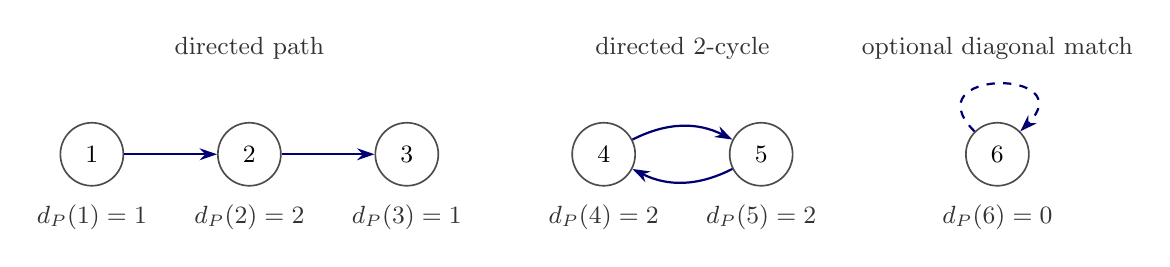
\begin{tikzpicture}[
  x=1cm,y=1cm,
  slot/.style={circle,draw=black!70,line width=.6pt,
    minimum size=8mm,inner sep=2pt,font=\small},
  edge/.style={-{Stealth[length=2.2mm,width=1.5mm]},
    draw=blue!45!black,line width=.8pt},
  note/.style={font=\small,align=center,text=black!80}
]
  \node[slot] (one) at (0,0) {$1$};
  \node[slot] (two) at (2,0) {$2$};
  \node[slot] (three) at (4,0) {$3$};
  \draw[edge] (one) -- (two);
  \draw[edge] (two) -- (three);
  \node[note] at (2,1.35) {directed path};
  \node[note] at (0,-.8) {$d_P(1)=1$};
  \node[note] at (2,-.8) {$d_P(2)=2$};
  \node[note] at (4,-.8) {$d_P(3)=1$};

  \node[slot] (four) at (6.5,0) {$4$};
  \node[slot] (five) at (8.5,0) {$5$};
  \draw[edge] (four) to[bend left=27] (five);
  \draw[edge] (five) to[bend left=27] (four);
  \node[note] at (7.5,1.35) {directed $2$-cycle};
  \node[note] at (6.5,-.8) {$d_P(4)=2$};
  \node[note] at (8.5,-.8) {$d_P(5)=2$};

  \node[slot] (six) at (11.5,0) {$6$};
  \draw[edge,dashed] (six) to[out=135,in=45,looseness=5] (six);
  \node[note] at (11.5,1.35) {optional diagonal match};
  \node[note] at (11.5,-.8) {$d_P(6)=0$};
\end{tikzpicture}
\caption{A self-matching after identifying the two copies of the slot labels.
The solid edges form the off-diagonal matching
$P=\{(1,2),(2,3),(4,5),(5,4)\}$; each label has at most one incoming
and one outgoing edge. The degree $d_P(i)$ counts both.
A diagonal match is available only at an isolated label, as illustrated
by the optional dashed loop at $6$; even the degree-one path endpoints
cannot receive a diagonal match.}
\label{fig:self-matching}
\end{figure}


\subsection{Application to residual caps}

We return to the fixed parameters and the spherical intensity $\mu$
of Section~\ref{sec:construction}. The following consequence collects
the inputs needed for the target selection in the next section.

\begin{corollary}[Witnesses for residual lists]
\label{cor:witnesses}
Fix $A_0>0$. There are constants $A,C_*,H>0$ such that, for all
sufficiently large $n$, the following holds. Let $R\ge1$, and let
$(x_{\alpha i})_{i=1}^{m_\alpha}$, $\alpha\in\mathcal A$, be any
finite nonempty family of deterministic lists satisfying
\[
 1\le m_\alpha\le n^2,\qquad
 r_--3\eta\le |x_{\alpha i}|\le b+3\eta.
\]
Define
\[
 C_{\alpha i}=\{u\in S^{n-1}:|u\cdot x_{\alpha i}|>1+3\eta\},
 \qquad
 s_{\alpha i}=-\log\min\{\mu(C_{\alpha i}),1/2\},
\]
and suppose $m_\alpha+\sum_i s_{\alpha i}\le A_0R$.
For each list there is a nonempty block partition and measurable slots
$E_{\alpha S}\subseteq\bigcap_{i\in S}C_{\alpha i}$, chosen
independently of $\Pi$, with positive intensities at most $1/2$.
Their activities and diagrams satisfy
\begin{equation}
 e^{-AR}\le\nu_\alpha\le1,\qquad
 D_{\alpha\alpha}\le\nu_\alpha^2e^{C_*R}.
 \label{eq:witness-self}
\end{equation}
For distinct $\alpha,\beta$, if all cross-residual angles exceed
$H\sqrt{\log n/n}$, then
\begin{equation}
 D_{\alpha\beta}\le n^{-3}\nu_\alpha\nu_\beta.
 \label{eq:witness-cross}
\end{equation}
If all those angles exceed $4\sqrt\varepsilon$, then
$D_{\alpha\beta}=0$. A positive injection count for a list implies
that every cap in that list is hit by $\Pi$.
\end{corollary}

\begin{proof}
Apply Lemma~\ref{lem:caps} with shell parameter $10$ and perturbation
bound $3$. Its affinity and common-intersection estimates supply the
hypotheses of Proposition~\ref{prop:blocks}; the common-intersection
constant is available before the radius multiplier in that proposition
is fixed. Apply the proposition separately to each list, making all
choices before sampling $\Pi$. The budget
\eqref{eq:block-first-budget} gives
\[
 -\log\nu_\alpha
 \le\sum_S\log(1+\lambda_{\alpha S}^{-1})\le AR.
\]
Together with \eqref{eq:block-row-budget} and
\eqref{eq:self-diagram-product}, it also gives the self bound in
\eqref{eq:witness-self}, after choosing $C_*$.

To check the cross estimate, write
$\bar c_{\alpha i}=\min\{\mu(C_{\alpha i}),1/2\}$ and let
$i(S)$ be the anchor of a block. Lemma~\ref{lem:caps} and
Proposition~\ref{prop:blocks} provide fixed exponents $P_0,P_1>0$
such that
\[
 \bar c_{\alpha i}\ge n^{-P_0},\qquad
 \lambda_{\alpha S}\ge n^{-P_1}\bar c_{\alpha,i(S)},\qquad
 E_{\alpha S}\subseteq C_{\alpha,i(S)}.
\]
Apply the affinity estimate to each two-element list of anchor residuals;
this does not require the union of the two full lists to have at most
$n^2$ entries. It gives
\[
 \frac{\mu(E_{\alpha S}\cap E_{\beta T})}
      {\lambda_{\alpha S}\lambda_{\beta T}}
 \le Cn^{2P_1+P_0}
       e^{-c n\angle(x_{\alpha,i(S)},x_{\beta,i(T)})^2}.
\]
There are at most $n^4$ block pairs. Choose $H$ after these constants,
so that $cH^2>9+2P_1+P_0$. For sufficiently large $n$, the angular
hypothesis gives $\rho_{\alpha\beta}\le n^{-4}$. Equation
\eqref{eq:cross-diagram-product} now gives
$D_{\alpha\beta}\le2n^{-4}\nu_\alpha\nu_\beta$, which implies
\eqref{eq:witness-cross}. At cross angles greater than
$4\sqrt\varepsilon$, Corollary~\ref{cor:caps-disjoint}
makes every cross-slot intersection empty, and the diagram is zero.

Finally, the point assigned to a block lies in every cap belonging to
that block. A positive injection count thus hits every residual cap.
\end{proof}

For a finite center list $(p_i)$ and a target $y$, take all residuals
$x_i=y-p_i$ with $|x_i|\le b+3\eta$. If this list satisfies the
hypotheses of Corollary~\ref{cor:witnesses}, a positive witness excludes
each such residual from $K^+$ by a strict slab inequality. All remaining
residuals are excluded by its outer ball. Consequently
\begin{equation}
 Z_y>0\quad\Longrightarrow\quad
 y\notin\bigcup_i(p_i+K^+).
 \label{eq:witness-hole}
\end{equation}
If the relevant list is empty, the target is already a hole.
Proposition~\ref{prop:poisson} supplies an exponential bound on the
probability that every chosen target lacks a witness. A second-moment
bound alone would not give the decay required for the finite-pattern
union in the final argument.

\section{Many targets for each finite pattern}
\label{sec:targets}

We now fix one of the rounded center lists supplied by
Proposition~\ref{prop:localization}.  Our goal is to bound the probability
that this list covers the window $B_D$ by translates of $K^+$.
The good subset of the window contains many points whose residual vectors
are separated at a small angular scale.  Only a small fraction of pairs
need fail a larger, fixed separation.  The former property controls every
cross diagram; the latter makes most cross diagrams vanish.

\subsection{A deterministic choice of targets}

The following volume estimate controls projective angles, including both
possible orientations of a residual vector.

\begin{lemma}[Cylinder estimate]
\label{lem:cylinder}
Let $n\ge2$, let $D,L>0$, and let $G\subset B_D$ be measurable with
$|G|\ge\omega_nD^n/4$.  Let $Y,Z$ be independent uniform points of $G$,
and let $p,q\in\mathbb R^n$.  For $0<\xi<\pi/2$,
\begin{align}
&\mathbb P\bigl(0<|Y-p|\le L,\ 0<|Z-q|\le L,
                 \ \angle(Y-p,Z-q)\le\xi\bigr)
\notag\\[-2pt]
&\hspace{30mm}\le
 8\frac{\omega_{n-1}}{\omega_n}
       \left(\frac{L\sin\xi}{D}\right)^{n-1}
 \le 8\sqrt n\left(\frac{L\sin\xi}{D}\right)^{n-1}.
\label{eq:cylinder}
\end{align}
\end{lemma}

\begin{proof}
Condition on $Y=y$ with $0<|y-p|\le L$, and write
$u=(y-p)/|y-p|$.  If the event in the statement occurs, the component
of $Z-q$ perpendicular to $u$ has length at most $L\sin\xi$.
Both orientations allowed by the projective angle therefore lie in the
same cylinder around the affine line $q+\mathbb Ru$.
The projection of $B_D$ onto the direction $u$ has length $2D$.
Every perpendicular slice of the cylinder has $(n-1)$-dimensional volume
at most $\omega_{n-1}(L\sin\xi)^{n-1}$.  Thus the allowed points $Z$
have volume at most $2D\omega_{n-1}(L\sin\xi)^{n-1}$.
Divide by $|G|$ and then average over $Y$.

To obtain the last inequality, use the slicing identity
\[
 \frac{\omega_n}{\omega_{n-1}}
 =\int_{-1}^1(1-t^2)^{(n-1)/2}\,dt
 \ge\frac{2\exp(-1/2)}{\sqrt n}.
\]
Indeed, restrict the integral to $|t|\le n^{-1/2}$ and use
$\log(1-1/n)\ge-1/(n-1)$.  In particular,
$\omega_{n-1}/\omega_n\le\sqrt n$.
\end{proof}

For a finite center list $P=(p_1,\ldots,p_N)$ and a point $y$ different
from its entries, write
\[
 \mathcal R_P(y)=(y-p_i:\ |y-p_i|\le b+3\eta)
\]
for its labeled list of relevant residuals.  For $\xi>0$, call a pair
$(y,z)$ \emph{$\xi$-bad} if some residual in $\mathcal R_P(y)$ and
some residual in $\mathcal R_P(z)$ have projective angle at most $\xi$.
This definition is symmetric in $y,z$ and retains repeated center labels.
Recall $\gamma$ from \eqref{eq:rates}, and put
\begin{equation}
 M_n=\left\lfloor\exp\left(\frac{n\log n}{16}\right)\right\rfloor.
\label{eq:target-count}
\end{equation}

\begin{lemma}[Separated targets]
\label{lem:targets}
Fix $H>0$ and $k_0>0$.  For all sufficiently large $n$, let
$P=(p_1,\ldots,p_N)$ be a deterministic list satisfying
\[
 N\le n^{k_0}\exp(\lambda_0n),
\]
and let $G\subset B_D\setminus\{p_1,\ldots,p_N\}$ be measurable with
$|G|\ge\omega_nD^n/4$.
There are $M_n$ distinct points $y_1,\ldots,y_{M_n}\in G$ such that:
\begin{enumerate}[label=\textup{(\roman*)}]
\item no pair with distinct indices is
$H\sqrt{\log n/n}$-bad;
\item at most a fraction $10f_n$ of the unordered pairs with distinct
indices is $4\sqrt\varepsilon$-bad, where
\begin{equation}
 f_n=8\sqrt n\,n^{2k_0}\exp(2\lambda_0n)
       \left(\frac{8\sqrt\varepsilon}{D}\right)^{n-1}
     =\exp\bigl(-\gamma n+O(\log n)\bigr).
\label{eq:bad-pair-rate}
\end{equation}
\end{enumerate}
The constants and the dimension threshold are uniform in $P$ and $G$.
The selected points can be fixed using only $P$ and $G$.
\end{lemma}

\begin{proof}
Sample $M_n$ points independently and uniformly from $G$.
For independent sampled points $Y,Z$, take the union in
Lemma~\ref{lem:cylinder} over all $N^2$ ordered pairs of center labels.
Since $b+3\eta\le2$ for sufficiently large $n$, this gives
\begin{equation}
 \mathbb P\bigl((Y,Z)\text{ is $\xi$-bad}\bigr)
 \le8\sqrt n\,N^2
       \left(\frac{2\sin\xi}{D}\right)^{n-1}.
\label{eq:target-pair}
\end{equation}
All relevant labels are included even though the relevant lists vary
with $Y$ and $Z$.  Repeated centers only repeat events in this union.

Set $t_n=H\sqrt{\log n/n}$.  Multiply the right side of
\eqref{eq:target-pair}, with $\sin t_n\le t_n$, by
$\binom{M_n}{2}$.  The logarithm of the resulting bound is at most
\[
 -\frac38n\log n+\frac12n\log\log n+O_{H,k_0}(n),
\]
which tends to $-\infty$.  Thus the probability that any pair of
sampled points is $t_n$-bad tends to zero, uniformly in the pattern.
For $\xi=4\sqrt\varepsilon$, the inequality
$\sin\xi\le4\sqrt\varepsilon$ instead bounds
\eqref{eq:target-pair} by $f_n$.
The expected fraction of these bad unordered pairs is at most $f_n$.
Markov's inequality shows that this fraction exceeds $10f_n$ with
probability at most $1/10$.
Consequently both conclusions hold with probability at least
$9/10-o(1)>0$.  The sampled points are distinct almost surely because
uniform measure on $G$ has no atoms.  Fix a successful list.
No independence between the two separation properties is needed.
\end{proof}

\subsection{From targets to a small covering probability}

We apply the preceding selection before exposing the Poisson process.
For each selected target, Corollary~\ref{cor:witnesses} supplies sets of
slab normals whose simultaneous occupancy certifies that the target is
uncovered.  Binning their activities will let us combine many certificates
without losing their angular separation.

\begin{proposition}[Failure probability for one pattern]
\label{prop:pattern-tail}
There are constants $c_0,C_{\mathrm{tail}}>0$ and $n_0$ such that, whenever
$n\ge n_0$ and $1\le R\le c_0n\log n$, every retained pattern
$P\in\mathcal F_n$ of Proposition~\ref{prop:localization} satisfies
\begin{equation}
 \mathbb P\left(B_D\subseteq\bigcup_{p\in P}(p+K^+)\right)
 \le \exp\left[-\exp\bigl(\gamma n-C_{\mathrm{tail}}\log n\bigr)\right].
\label{eq:pattern-tail}
\end{equation}
The constants are independent of the pattern, its repetitions, and $R$.
\end{proposition}

The covering event is measurable. Indeed, the finite union of translates
of $K^+$ is closed, so it covers $B_D$ exactly when it contains a fixed
countable dense subset of $B_D$. At each such point, membership is a
finite union of ball conditions and Poisson cap-avoidance events.

\begin{proof}
Fix $P\in\mathcal F_n$ and its deterministic good set $G_P$.
At each $y\in G_P$, Proposition~\ref{prop:localization} gives
\begin{equation}
 r_--2\eta\le |x_i|\le b+3\eta,\qquad
 m_y\le2C_{\mathrm{loc}}R,\qquad
 \sum_{i=1}^{m_y}w_a(|x_i|)\le2C_{\mathrm{loc}}R
\label{eq:target-residual-budget}
\end{equation}
for its relevant residuals $x_i=y-p_i$.
If this list is empty at any point of $G_P$, that point lies in none of
the balls $p+(b+3\eta)B$, so the probability in
\eqref{eq:pattern-tail} is zero.  We may assume all these lists are
nonempty.  For the range of $R$ in the proposition,
$m_y\le n^2$ once $n$ is sufficiently large.

For each relevant residual, define the cutting cap
\[
 C_i(y)=\{u\in S^{n-1}:|u\cdot x_i|>1+3\eta\}.
\]
Lemma~\ref{lem:caps}, applied with radial loss $10\log n/n$
and a fixed perturbation bound, gives
\[
 s_i=-\log\min\{\mu(C_i(y)),1/2\}
       \le C_a w_a(|x_i|).
\]
Consequently
\begin{equation}
 m_y+\sum_{i=1}^{m_y}s_i\le A_0R,
 \qquad A_0=2C_{\mathrm{loc}}(1+C_a).
\label{eq:target-cap-budget}
\end{equation}
All assumptions of Corollary~\ref{cor:witnesses}
therefore hold uniformly in $y$ and $P$.  Fix its constants $A,C_*$ and
$H$ for this value of $A_0$.

The list-length estimate in Proposition~\ref{prop:localization} gives
$N\le n^{k_0}\exp(\lambda_0n)$ for a fixed $k_0$, uniformly in the
present range of $R$.  Apply Lemma~\ref{lem:targets} to $G_P$ with the
just-fixed $H$.  At each of the resulting $M=M_n$ targets, choose the
block partition and measurable witness sets from
Corollary~\ref{cor:witnesses}.  Denote its injection count by $Z_y$,
its activity by $\nu_y$, and the diagram sums by $D_{yz}$.
The corollary gives
\begin{equation}
 \exp(-AR)\le\nu_y\le1,
 \qquad D_{yy}\le\nu_y^2\exp(C_*R).
\label{eq:target-activities}
\end{equation}
Every pair of distinct selected targets satisfies
$D_{yz}\le n^{-3}\nu_y\nu_z$.
Moreover, $D_{yz}=0$ unless the pair is $4\sqrt\varepsilon$-bad.
Our use of ``at most'' in the definition of badness makes both angular
interfaces strict on its complement.

All choices so far depend only on $P$ and its targets.  In particular,
the witness sets are chosen before the Poisson process; their activities
are deterministic intensities.  There is no need to choose witness sets
measurably at every point of $G_P$, since only the finite selected list
is used.  If $Z_y>0$, every relevant residual is cut by a slab of the
process, and the other centers are too far from $y$ to contain it in a
translate of $K^+$.  Thus $Z_y>0$ certifies a hole.

Divide the possible values of $-\log\nu_y$ in $[0,AR]$ into intervals
of length $\log2$.  At most
\[
 Q=1+\left\lceil\frac{AR}{\log2}\right\rceil
\]
bins suffice.  A largest bin has $m\ge M/Q$ targets and, for some
$\nu>0$, all its activities belong to $[\nu,2\nu]$.
There are at most $10f_n\binom M2$ bad unordered pairs in the full
list.  Hence the chosen bin contains at most
\begin{equation}
 10f_nM(M-1)\le10f_nQ^2m^2
\label{eq:bin-bad-pairs}
\end{equation}
bad ordered pairs with distinct indices.
This bound allows the bin to contain every bad pair; no independence
between bin membership and angles is asserted.

Apply Proposition~\ref{prop:poisson} to the witnesses in this bin.
Its numerator is at least $m^2\nu^2$.  By
\eqref{eq:target-activities} and \eqref{eq:bin-bad-pairs}, its denominator
before the factor $2$ is at most
\[
 \sum_{y,z}D_{yz}
 \le4m\nu^2\exp(C_*R)
       +40m^2\nu^2n^{-3}Q^2f_n.
\]
The first term counts diagonal pairs.  Among distinct pairs, only the
coarse bad pairs contribute.  Coverage forces $Z_y=0$ at every target
of the bin, so
\begin{equation}
 \mathbb P\left(B_D\subseteq\bigcup_{p\in P}(p+K^+)\right)
 \le\exp\left[-\frac1{
 8\bigl(\exp(C_*R)/m+10n^{-3}Q^2f_n\bigr)}\right].
\label{eq:bin-tail}
\end{equation}

Now choose
\[
 c_0=\frac1{64\max\{C_*,1\}}.
\]
Uniformly for $1\le R\le c_0n\log n$, we have $\log Q=O(\log n)$ and,
for sufficiently large $n$,
\[
 m\exp(-C_*R)
 \ge\frac{M_n}{Q}\exp(-C_*R)
 \ge\exp\left(\frac{n\log n}{32}\right).
\]
The first term inside the parentheses in \eqref{eq:bin-tail} is
therefore at most $\exp(-n\log n/32)$.  By
\eqref{eq:bad-pair-rate}, the second is
$\exp(-\gamma n+O(\log n))$.
Since $\gamma$ is fixed, their sum is at most
$\exp(-\gamma n+O(\log n))$; absorbing the fixed factor $8$ gives
\eqref{eq:pattern-tail}.

The order of the choices is fixed throughout: the geometric parameters
come first, then the cap and block constants and $H$, then $c_0$, and
finally the dimension threshold.  Every estimate is uniform over the
retained finite class.  In particular, the auxiliary target selection
introduces no dependence on the realization of $\Pi$.
\end{proof}

\section{Completion of the proof}\label{sec:assembly}

We now combine the estimates and specify their order of use. The numerical
parameters~\eqref{eq:fixed-constants} are already fixed. Apply
Lemma~\ref{lem:caps} with the shell and perturbation constants required by
Proposition~\ref{prop:localization}. Its affinity and common-intersection
constants determine the constants in Proposition~\ref{prop:blocks},
including its radius cutoff. The radial cost estimate gives
$A_0=2C_{\mathrm{loc}}(1+C_a)$ in the residual budget.
For this value of $A_0$, Corollary~\ref{cor:witnesses} fixes the
cross-angle constant $H$ and the self-diagram coefficient $C_*$.
Choose a positive rational number
\begin{equation}\label{eq:choose-c}
 c\le\frac1{64\max(C_*,1)}.
\end{equation}
Every constant in this order is independent of dimension. Increase $n_0$
so that all preceding estimates hold when $n\ge n_0$ and
$R=c n\log n$. In particular, $R\ge1$, $R\le n^2$, and every relevant cap
list has at most $n^2$ entries.

\begin{proof}[Proof of Theorem~\ref{thm:main}]
Use the deterministic class $\mathcal F_n$ from
Proposition~\ref{prop:localization}, with $R=c n\log n$. That proposition
and Proposition~\ref{prop:pattern-tail} give
\begin{align*}
 &\mathbb P\left\{\text{some }P\in\mathcal F_n
             \text{ covers }B_D\text{ by translates of }K^+\right\}\\
 &\hspace{1cm}\le
 \exp\left(\exp(\lambda_0 n+O(\log n))
                -\exp(\gamma n-O(\log n))\right)=o(1).
\end{align*}
The error bounds are uniform over this finite class. Since
$\gamma>\lambda_0$, the negative term dominates. Lemma~\ref{lem:volume}
therefore guarantees a realization for which $|K|>2v\omega_n a^n$ and
no retained pattern covers $B_D$ by translates of $K^+$.

Suppose that $K+\Lambda+T=\mathbb R^n$ with
$|T|/\det\Lambda\le\rho_0$. Proposition~\ref{prop:localization} would give
a retained pattern covering $B_D$ by $K^+$, a contradiction. Every covering
thus has center intensity greater than $\rho_0$. Taking the infimum of
its density yields
\[
 \theta_T(K)=\theta_{\mathrm{per}}(K)\ge\rho_0|K|>R=c n\log n,
\]
where Proposition~\ref{prop:periodization} supplies the equality.
The realization is a centrally symmetric convex body, as observed after
\eqref{eq:buffered-body}. Choose one for each $n\ge n_0$.
\end{proof}

The exclusion is simultaneous over all full-rank lattices and all finite
coset lists. The lattice and the centers may depend on the chosen body:
localization still places their rounded list in the class fixed before
sampling. The periodization equivalence transfers this exclusion to
unrestricted locally finite coverings without changing the body or the
constant.

\subsection{The optimal order for translative and lattice coverings}

For a convex body $K$, define its single-lattice covering density by
\[
 \theta_L(K)=\inf_{\Lambda:\ K+\Lambda=\mathbb R^n}
                   \frac{\vol(K)}{\det\Lambda}.
\]
Every lattice covering is periodic, so
$\theta_T(K)=\theta_{\mathrm{per}}(K)\le\theta_L(K)$.
Let $\mathcal K^n$ denote the convex bodies in $\mathbb R^n$ and
$\mathcal K^n_{\mathrm{sym}}$ their centrally symmetric members.

\begin{corollary}\label{cor:sharp-order}
As $n\to\infty$, each of the four quantities
\begin{gather*}
 \sup_{K\in\mathcal K^n}\theta_T(K),\qquad
 \sup_{K\in\mathcal K^n_{\mathrm{sym}}}\theta_T(K),\\
 \sup_{K\in\mathcal K^n}\theta_L(K),\qquad
 \sup_{K\in\mathcal K^n_{\mathrm{sym}}}\theta_L(K)
\end{gather*}
has order $n\log n$, with absolute comparison constants.
\end{corollary}
\begin{proof}
Theorem~\ref{thm:main} gives the lower bound already among centrally
symmetric bodies, and $\theta_T\le\theta_L$ transfers it to lattice
coverings. Rogers' bound~\eqref{eq:rogers} supplies the translative upper
bound. The companion single-lattice theorem
\cite[Theorem~1.1]{OpenAI2026SingleLattice} gives
$\theta_L(K)\le Cn\log n$ for every convex body and every $n\ge2$,
which supplies the two lattice upper bounds.
\end{proof}

\section{Rational polytopes and normal lists}\label{sec:encoding}

The strict volume margin in the proof gives a polyhedral consequence of
Theorem~\ref{thm:main} without changing its constant.

\begin{corollary}\label{cor:rational-polytope}
With the same $c$ and $n_0$ as in Theorem~\ref{thm:main}, for every
$n\ge n_0$ there is a centrally symmetric polytope
$P_n\subset\mathbb R^n$ with rational vertices such that
\[
 \theta_T(P_n)>c n\log n.
\]
\end{corollary}
\begin{proof}
Fix the successful body $K$ in the proof of Theorem~\ref{thm:main},
and put $R=c n\log n$. It satisfies
$|K|>2v\omega_na^n$, and no periodic covering by $K$ has center
intensity at most $\rho_0=R/(2v\omega_na^n)$.

Enumerate the rational points of $\operatorname{int}K$ as
$q_1,q_2,\ldots$ and set
\[
 P_j=\operatorname{conv}\{\pm q_1,\ldots,\pm q_j\}.
\]
These are centrally symmetric rational polytopes contained in
$\operatorname{int}K$, and they increase with $j$. Their union is
$\operatorname{int}K$: every interior point lies inside a sufficiently
small simplex with rational vertices in $\operatorname{int}K$, and
all its vertices eventually occur in the enumeration. Continuity of
volume from below, together with the fact that the boundary of a convex
body has measure zero, gives $|P_j|\to|K|$. Choose $j$ so that
$|P_j|>2v\omega_na^n$; in particular, this $P_j$ has nonempty interior.

Every periodic covering by $P_j$ is a covering by $K$, because
$P_j\subset K$. Its center intensity therefore exceeds $\rho_0$.
Taking the infimum of the covering densities and using
Proposition~\ref{prop:periodization} yields
\[
 \theta_T(P_j)=\theta_{\mathrm{per}}(P_j)
       \ge\rho_0|P_j|>R.
\]
This argument uses both inclusion and the retained volume margin.
\end{proof}

A different finite description retains the spherical truncation $bB$
and makes all slab normals rational unit vectors. These bodies need not
be polytopes.

\begin{proposition}\label{prop:rational}
The bodies in Theorem~\ref{thm:main} can be chosen in the form
\[
 K=bB\cap\bigcap_{j=1}^m\{x:|u_j\cdot x|\le1\},
 \qquad u_j\in\mathbb Q^n\cap S^{n-1},
\]
with $m<\infty$.
\end{proposition}
\begin{proof}
Fix a successful finite normal list $U=(u_1,\ldots,u_m)$ from the proof of
Theorem~\ref{thm:main}. The class $\mathcal F_n$ is finite and independent
of $U$. For each $P\in\mathcal F_n$, select a point $y_P\in B_D$ outside
all of its translates of $K^+(U)$. For every center $p$ in that list,
either $|y_P-p|>b+3\eta$, or one of the normals satisfies
\[
 |u_j\cdot(y_P-p)|>1+3\eta.
\]
Each required inequality is strict. There are finitely many patterns,
centers, and chosen certificates, so all these inequalities persist under
a sufficiently small simultaneous perturbation of the normals. Empty
patterns need no certificates.

The strict volume test persists as well. If $U'$ is a list of unit normals
with $|u_j-u'_j|\le\delta$ for every $j$, then
\begin{equation}\label{eq:volume-continuity}
 (1+b\delta)^{-1}K(U)\subset K(U')\subset(1+b\delta)K(U).
\end{equation}
Indeed, if $x\in K(U)$, then $|x|\le b$ and
$|u'_j\cdot x|\le1+b\delta$; scaling by $(1+b\delta)^{-1}$ proves the
first inclusion. Interchanging $U$ and $U'$ proves the second. Volumes
therefore converge as $\delta\to0$.

Rational unit vectors are dense in $S^{n-1}$ for $n\ge2$, by the
stereographic parametrization
\[
 t\longmapsto\frac{(2t,1-|t|^2)}{1+|t|^2},
 \qquad t\in\mathbb Q^{n-1},
\]
and approximation of its omitted pole. Approximate all normals closely
enough to preserve the holes and the strict volume test. The localization
argument applies to every finite normal list, so the resulting rational
list yields the same lower bound.

\end{proof}

One can specify a choice exactly by ordering the finite rational normal
lists. Write each coordinate in reduced form with positive denominator,
and let its height be the maximum of the absolute numerator and denominator.
Order lists by their length plus maximum coordinate height (height $1$
for the empty list), breaking each finite tie lexicographically.
The lists satisfying the strict volume test and every finite-pattern
noncoverage test form a nonempty set, so they have a first member.
This specifies a finite mathematical object; it does not assert an
algorithm for deciding the volume comparisons or an effective bound for
the first admissible dimension.

\appendix
\section{Covering density and periodization}
\label{sec:periodization}

The proof constructs bodies that exclude every finite union of lattice
cosets. We verify that this gives the same lower bound for unrestricted
translative coverings, with a precise density convention. This standard
periodization principle is recorded in Prosanov~\cite[Theorem~2.1]{Prosanov2021PackingCovering},
with attribution to Rogers. We give the finite-window argument to make
its boundary and limiting conventions explicit.

Fix a convex body $K\subset\mathbb R^n$ and write $V=\vol(K)$.
Use the definitions of $\theta_T$ and $\theta_{\mathrm{per}}$ from
Section~1. For a locally finite covering center set $X$, the centered
cube lower density replaces the $\limsup$ in
\eqref{eq:unrestricted-density} by $\liminf$. The centered ball
versions use $B_R$ and $\vol(B_R)$ in place of $Q_R$ and $(2R)^n$.

\begin{proposition}[Periodization]
\label{prop:periodization}
For every convex body $K\subset\mathbb R^n$,
\[
 \theta_T(K)=\theta_{\mathrm{per}}(K).
\]
The same infimum is obtained by replacing the centered cube upper density
by centered cube lower density or centered Euclidean-ball lower or upper
density. These are equalities of infima over coverings; the corresponding
statistics of one covering need not agree.
\end{proposition}

\begin{proof}
Choose $r>0$ with $K\subset Q_r$, and let $X$ be a locally finite
covering center set. For $a\in\mathbb R^n$ and $L>0$, the finite set
\[
 S=X\cap(a+Q_{L+r})
\]
covers $a+Q_L$ by translates of $K$. Indeed, if $y\in a+Q_L$ and
$y=k+x$ with $k\in K$ and $x\in X$, then $x=y-k\in a+Q_{L+r}$.
This holds on the boundary as well. Repeating $S$ with periods
$2L\mathbb Z^n$ covers all of $\mathbb R^n$ because the cubes
$a+Q_L+2Lz$ cover it. Reducing $S$ modulo this lattice gives
\begin{equation}
 \theta_{\mathrm{per}}(K)
 \le \frac{V\#(X\cap(a+Q_{L+r}))}{(2L)^n}.
 \label{eq:density-window}
\end{equation}
Writing $R=L+r$, we obtain, for every $a$ and every $R>r$,
\begin{equation}
 \frac{V\#(X\cap(a+Q_R))}{(2R)^n}
 \ge \theta_{\mathrm{per}}(K)(1-r/R)^n.
 \label{eq:density-cubes}
\end{equation}
This proves the required lower bound for both centered cube conventions.

For the ball conventions, fix $L>0$ and put
$\beta=\sqrt n(L+r)$. Integrate \eqref{eq:density-window} over
$a\in z+B_{R-\beta}$, where $R>\beta$. Any counted center belongs to $z+B_R$,
and each such center is counted on a set of $a$ of volume at most
$(2(L+r))^n$. Tonelli's theorem therefore gives
\[
 \frac{\theta_{\mathrm{per}}(K)(2L)^n}{V}\vol(B_{R-\beta})
 \le \int_{z+B_{R-\beta}}\#(X\cap(a+Q_{L+r}))\,da
 \le (2(L+r))^n\#(X\cap(z+B_R)).
\]
Consequently, uniformly in $z$,
\[
 \frac{V\#(X\cap(z+B_R))}{\vol(B_R)}
 \ge \theta_{\mathrm{per}}(K)
       \left(\frac{L}{L+r}\right)^n(1-\beta/R)^n.
\]
First let $R\to\infty$ with $L$ fixed, and then let $L\to\infty$.
This proves the lower bound for the ball lower densities and hence also
for the upper densities. No comparison of a ball with just one
containing or contained cube is needed.

For the reverse inequality, consider a periodic center set
$X=\Lambda+T$ with distinct cosets. Let $F$ be a bounded half-open
fundamental parallelepiped of $\Lambda$ and choose $d>0$ with
$F\subset Q_d\cap B_d$. For each fixed $t\in T$, the cells
$t+\lambda+F$ partition space up to null boundaries. For $R>d$ and
$W_R=Q_R$ or $B_R$, the cells based at points of $t+\Lambda$ in
$z+W_R$ contain $z+W_{R-d}$ up to a null set and are contained in
$z+W_{R+d}$. Thus
\[
 \vol(W_{R-d})\le
 \det\Lambda\,\#((t+\Lambda)\cap(z+W_R))
 \le\vol(W_{R+d}).
\]
Divide by $\vol(W_R)$ and sum over the distinct cosets. Every stated
center-count intensity is therefore $|T|/\det\Lambda$, uniformly in $z$;
the corresponding covering density is $V|T|/\det\Lambda$.
The finite constant $d$ may depend on the lattice; no bound uniform over
lattices is needed. Since periodic center sets are locally finite,
restricting each unrestricted infimum to these competitors proves the
reverse inequality.
\end{proof}

\paragraph{Average overlap multiplicity.}
One customary definition uses the lower ball density of the overlap
multiplicity~\cite[Section~1.1]{Prosanov2021PackingCovering}. It agrees
with the convention above. For either choice of $W_R$, put
\[
 A_W(X,R)=\sum_{x\in X}\vol((K+x)\cap W_R).
\]
Choose $s>0$ such that $K$ is contained in the radius-$s$ ball of the
norm defining $W_R$. Local finiteness gives, for $R>s$,
\[
 V\#(X\cap W_{R-s})\le A_W(X,R)
 \le V\#(X\cap W_{R+s}).
\]
Replacing $R$ by $R+s$ or $R-s$ does not change the liminf or limsup of
$\#(X\cap W_R)/\vol(W_R)$: substitute the shifted radius and use
$(R\pm s)^n/R^n\to1$. The lower and upper limits of
$A_W(X,R)/\vol(W_R)$ therefore equal the corresponding center-count intensities
multiplied by $V$. This counts each overlapping translate separately;
the volume of the covered union is not the density.

\paragraph{Transfer of the lower bound.}
In particular, any inequality $\theta_{\mathrm{per}}(K)>R$ established
by the finite-coset argument implies $\theta_T(K)>R$ for the same body
and the same constant. This uses equality of the infima and makes no
claim that an individual covering can be repeated at exactly its original
density. For every $\epsilon>0$, a covering of finite density $D$
does imply existence of a periodic covering of density less than
$D+\epsilon$.

\begingroup
\raggedright
\bibliographystyle{plain}
\bibliography{references}
\endgroup
\end{document}
